\documentclass{vkr}
\usepackage[english, russian]{babel} % переносы
\usepackage{graphicx} % для вставки картинок
\graphicspath{{images/}} % путь к изображениям
\usepackage[hidelinks]{hyperref}
\usepackage{float} % определяет метод H для рисунка с переносом на следующую страницу, ели не помещается
\usepackage{pdflscape}
\addto{\captionsrussian}{\renewcommand{\refname}{СПИСОК ИСПОЛЬЗОВАННЫХ ИСТОЧНИКОВ}}
\usepackage{xltabular} % для вставки таблиц
\usepackage{makecell}
\renewcommand\theadfont{} % шрифт в /thead
\usepackage{array} % для определения новых типов столбцов таблиц
\newcolumntype{T}{>{\centering\arraybackslash}X} % новый тип столбца T - автоматическая ширина столбца с выравниванием по центру
\newcolumntype{R}{>{\raggedleft\arraybackslash}X} % новый тип столбца R - автоматическая ширина столбца с выравниванием по правому краю
\newcolumntype{C}[1]{>{\centering\let\newline\\\arraybackslash\hspace{0pt}}m{#1}} % новый тип столбца C - фиксированная ширина столбца с выравниванием по центру
\newcolumntype{r}[1]{>{\raggedleft\arraybackslash}p{#1}} % новый тип столбца r - фиксированная ширина столбца с выравниванием по правому краю
\newcommand{\centrow}{\centering\arraybackslash} % командой \centrow можно центрировать одну ячейку (заголовок) в столбце типа X или p, оставив в оcтальных ячейках другой тип выравнивания
\newcommand{\finishhead}{\endhead\hline\endlastfoot}
\newcommand{\continuecaption}[1]{\captionsetup{labelformat=empty} \caption[]{#1}\\ \hline }
\usepackage{etoolbox}
\AtBeginEnvironment{xltabular}{\refstepcounter{tablecnt}} % подсчет таблиц xltabular, обычные таблицы подсчитываются в классе

\usepackage[tableposition=top]{caption} % подпись таблицы вверху
\captionsetup{strut=off}
\setlength{\intextsep}{0pt} % Vertical space above & below [h] floats
\setlength{\textfloatsep}{0pt} % Vertical space below (above) [t] ([b]) floats
\DeclareCaptionLabelFormat{gostfigure}{Рисунок #2} %подпись рисунка
\DeclareCaptionLabelFormat{gosttable}{Таблица #2} %подпись таблицы
\DeclareCaptionLabelSeparator{gost}{~--~} %разделитель в рисунках и таблицах
\captionsetup{labelsep=gost}
\captionsetup[figure]{aboveskip=10pt,belowskip=4mm,justification=centering,labelformat=gostfigure} % настройка подписи рисунка
\captionsetup[table]{font={stretch=1.41},skip=0pt,belowskip=0pt,aboveskip=8.5pt,singlelinecheck=off,labelformat=gosttable} % настройка подписи таблицы

\setlength{\LTpre}{8mm} % отступ сверху таблицы
\setlength{\LTpost}{6mm} % отступ снизу таблицы

\usepackage{enumitem}
\setlist{nolistsep,wide=\parindent,itemindent=*} % отступы вокруг списков, выравнивание с учетом разделителя

\usepackage{color} %% это для отображения цвета в коде
\usepackage{listings} %% листинги кода
\setmonofont[Scale=0.7]{Verdana} % моноширный шрифт для листинга

\definecolor{codegreen}{rgb}{0,0.6,0}
\definecolor{codegray}{rgb}{0.5,0.5,0.5}
\definecolor{codepurple}{rgb}{0.58,0,0.82}

\lstset{ %
language=C,                 % выбор языка для подсветки (здесь это С)
numbers=left,               % где поставить нумерацию строк (слева\справа)
numberstyle=\tiny,           % размер шрифта для номеров строк
stepnumber=1,                   % размер шага между двумя номерами строк
numbersep=5pt,                % как далеко отстоят номера строк от подсвечиваемого кода
commentstyle=\color{codegreen},
keywordstyle=\color{magenta},
numberstyle=\tiny\color{codegray},
stringstyle=\color{codepurple},
basicstyle=\linespread{0.95}\ttfamily,
backgroundcolor=\color{white}, % цвет фона подсветки - используем \usepackage{color}
showspaces=false,            % показывать или нет пробелы специальными отступами
showstringspaces=false,      % показывать или нет пробелы в строках
showtabs=false,             % показывать или нет табуляцию в строках
frame=single,              % рисовать рамку вокруг кода
tabsize=2,                 % размер табуляции по умолчанию равен 2 пробелам
captionpos=t,              % позиция заголовка вверху [t] или внизу [b] 
breaklines=true,           % автоматически переносить строки (да\нет)
breakatwhitespace=false, % переносить строки только если есть пробел
escapeinside={\%*}{*)}   % если нужно добавить комментарии в коде
}

\makeatletter % чтобы допускались русские комментарии в листингах
\lst@InputCatcodes
\def\lst@DefEC{%
 \lst@CCECUse \lst@ProcessLetter
  ^^80^^81^^82^^83^^84^^85^^86^^87^^88^^89^^8a^^8b^^8c^^8d^^8e^^8f%
  ^^90^^91^^92^^93^^94^^95^^96^^97^^98^^99^^9a^^9b^^9c^^9d^^9e^^9f%
  ^^a0^^a1^^a2^^a3^^a4^^a5^^a6^^a7^^a8^^a9^^aa^^ab^^ac^^ad^^ae^^af%
  ^^b0^^b1^^b2^^b3^^b4^^b5^^b6^^b7^^b8^^b9^^ba^^bb^^bc^^bd^^be^^bf%
  ^^c0^^c1^^c2^^c3^^c4^^c5^^c6^^c7^^c8^^c9^^ca^^cb^^cc^^cd^^ce^^cf%
  ^^d0^^d1^^d2^^d3^^d4^^d5^^d6^^d7^^d8^^d9^^da^^db^^dc^^dd^^de^^df%
  ^^e0^^e1^^e2^^e3^^e4^^e5^^e6^^e7^^e8^^e9^^ea^^eb^^ec^^ed^^ee^^ef%
  ^^f0^^f1^^f2^^f3^^f4^^f5^^f6^^f7^^f8^^f9^^fa^^fb^^fc^^fd^^fe^^ff%
  ^^^^20ac^^^^0153^^^^0152%
  % Basic Cyrillic alphabet coverage
  ^^^^0410^^^^0411^^^^0412^^^^0413^^^^0414^^^^0415^^^^0416^^^^0417%
  ^^^^0418^^^^0419^^^^041a^^^^041b^^^^041c^^^^041d^^^^041e^^^^041f%
  ^^^^0420^^^^0421^^^^0422^^^^0423^^^^0424^^^^0425^^^^0426^^^^0427%
  ^^^^0428^^^^0429^^^^042a^^^^042b^^^^042c^^^^042d^^^^042e^^^^042f%
  ^^^^0430^^^^0431^^^^0432^^^^0433^^^^0434^^^^0435^^^^0436^^^^0437%
  ^^^^0438^^^^0439^^^^043a^^^^043b^^^^043c^^^^043d^^^^043e^^^^043f%
  ^^^^0440^^^^0441^^^^0442^^^^0443^^^^0444^^^^0445^^^^0446^^^^0447%
  ^^^^0448^^^^0449^^^^044a^^^^044b^^^^044c^^^^044d^^^^044e^^^^044f%
  ^^^^0401^^^^0451%
  %%%
  ^^00}
\lst@RestoreCatcodes
\makeatother


% Режим шаблона (должен быть включен один из трех)
%\ВКРtrue
\Практикаtrue
%\Курсоваяtrue

\newcommand{\Дисциплина}{<<Проектирование и архитектура программных систем>>} % для курсовой
\newcommand{\КодСпециальности}{09.03.04} % Курсовая
\newcommand{\Специальность}{Программная инженерия} % Курсовая
\newcommand{\Тема}{Интеллектуальная система для выявления заболеваний } % ВКР Курсовая
\newcommand{\ТемаВтораяСтрока}{сельскохозяйственных растений}
\newcommand{\ГдеПроводитсяПрактика}{ООО «Предприятие ВТИ-Сервис»} % для практики
\newcommand{\РуководительПрактПредпр}{Федосов Д. В.} % для практики
\newcommand{\ДолжнРуководительПрактПредпр}{директор} % для практики
\newcommand{\РуководительПрактУнивер}{Чаплыгин А. А.} % для практики
\newcommand{\ДолжнРуководительПрактУнивер}{к.т.н. доцент} % для практики
\newcommand{\Автор}{Н. М. Крюков}
\newcommand{\АвторРод}{Крюкова Н. М.}
\newcommand{\АвторПолностьюРод}{Крюкова Никиты Михайловича} % для практики
\newcommand{\Шифр}{21-06-0071}
\newcommand{\Курс}{4} % для практики
\newcommand{\Группа}{ПО-11б}
\newcommand{\Руководитель}{Р. А. Томакова} % для ВКР и курсовой
\newcommand{\Нормоконтроль}{А. А. Чаплыгин} % для ВКР
\newcommand{\ЗавКаф}{А. В. Малышев} % для ВКР
\newcommand{\ДатаПриказа}{«07» апреля 2023~г.} % для ВКР
\newcommand{\НомерПриказа}{1505-с} % для ВКР
\newcommand{\СрокПредоставления}{«13» июня 2023~г.} % для ВКР, курсового

\begin{document}
\maketitle
\ifПрактика{}\else{
   \newpage
\begin{center}
\large\textbf{Минобрнауки России}

\large\textbf{Юго-Западный государственный университет}
\vskip 1em
\normalsize{Кафедра программной инженерии}
\vskip 1em
\ifВКР{
        \begin{flushright}
        \begin{tabular}{p{.4\textwidth}}
        \centrow УТВЕРЖДАЮ: \\
        \centrow Заведующий кафедрой \\
        \hrulefill \\
        \setarstrut{\footnotesize}
        \centrow\footnotesize{(подпись, инициалы, фамилия)}\\
        \restorearstrut
        «\underline{\hspace{1cm}}»
        \underline{\hspace{3cm}}
        20\underline{\hspace{1cm}} г.\\
        \end{tabular}
        \end{flushright}
        }\fi
\end{center}
\vspace{1em}
  \begin{center}
  \large
\ifВКР{
ЗАДАНИЕ НА ВЫПУСКНУЮ КВАЛИФИКАЦИОННУЮ РАБОТУ
  ПО ПРОГРАММЕ БАКАЛАВРИАТА}
  \else
ЗАДАНИЕ НА КУРСОВУЮ РАБОТУ (ПРОЕКТ)
\fi
\normalsize
  \end{center}
\vspace{1em}
{\parindent0pt
  Студента \АвторРод, шифр\ \Шифр, группа \Группа
  
1. Тема «\Тема\ \ТемаВтораяСтрока»
\ifВКР{
утверждена приказом ректора ЮЗГУ от \ДатаПриказа\ № \НомерПриказа
}\fi.

2. Срок предоставления работы к защите \СрокПредоставления

3. Исходные данные для создания программной системы:

3.1. Перечень решаемых задач:}

\renewcommand\labelenumi{\theenumi)}

\begin{enumerate}
\item провести анализ предметной области;
\item  разработать концептуальную модель системы управления IT-ин\-фра\-струк\-турой предприятия на основе подхода к управлению и организации ИТ-услуг ITSM;
\item спроектировать программную систему управления IT-ин\-фра\-струк\-турой предприятия;
\item сконструировать и протестировать программную систему управления IT-инфраструктурой предприятия.
\end{enumerate}

{\parindent0pt
  3.2. Входные данные и требуемые результаты для программы:}

\begin{enumerate}
\item Входными данными для программной системы являются: данные
справочников комплектующих, конфигураций, ПО, критериев качества SLA,
ИТ-услуг, департаментов компании; технические данные ИТ-ресурсов; данные входящих заявок на ИТ-ресурсы; данные запросов поставщикам на комплектующие.
\item Выходными данными для программной системы являются: сформированные заявки на обслуживание ИТ-ресурсов; сформированные запросы на
закупку комплектующих; сведения о выполненных работах по заявкам; статусы заявок; выходные отчеты (инфографика) – по качеству услуг, по состоянию ИТ-ресурсов, по деятельности ИТ-отдела, по стоимости обслуживания
ИТ-ресурсов, воронка заявок.
\end{enumerate}

{\parindent0pt

  4. Содержание работы (по разделам):
  
  4.1. Введение.
  
  4.1. Анализ предметной области.
  
4.2. Техническое задание: основание для разработки, назначение разработки,
требования к программной системе, требования к оформлению документации.

4.3. Технический проект: общие сведения о программной системе, проект
данных программной системы, проектирование архитектуры программной системы, проектирование пользовательского интерфейса программной системы.

4.4. Рабочий проект: спецификация компонентов и классов программной системы, тестирование программной системы, сборка компонентов программной системы.

4.5. Заключение.

4.6. Список использованных источников.

5. Перечень графического материала:

\списокПлакатов

\vskip 2em
\begin{tabular}{p{6.8cm}C{3.8cm}C{4.8cm}}
Руководитель \ifВКР{ВКР}\else работы (проекта) \fi & \lhrulefill{\fill} & \fillcenter\Руководитель\\
\setarstrut{\footnotesize}
& \footnotesize{(подпись, дата)} & \footnotesize{(инициалы, фамилия)}\\
\restorearstrut
Задание принял к исполнению & \lhrulefill{\fill} & \fillcenter\Автор\\
\setarstrut{\footnotesize}
& \footnotesize{(подпись, дата)} & \footnotesize{(инициалы, фамилия)}\\
\restorearstrut
\end{tabular}
}

\renewcommand\labelenumi{\theenumi.}

   \abstract{РЕФЕРАТ}

Объем работы равен \formbytotal{lastpage}{страниц}{е}{ам}{ам}. Работа содержит \formbytotal{figurecnt}{иллюстраци}{ю}{и}{й}, \formbytotal{tablecnt}{таблиц}{у}{ы}{}, \arabic{bibcount} библиографических источников и \formbytotal{числоПлакатов}{лист}{}{а}{ов} графического материала. Количество приложений – 2. Графический материал представлен в приложении А. Фрагменты исходного кода представлены в приложении Б.

Перечень ключевых слов: коммерческий сайт, Система, CMS, Битрикс, Joomla, аддитивные технологии, 3D-принтеры, услуги, сервисы, информатизация, автоматизация, информационные технологии, веб-форма,  Apache, классы, база данных, средства защиты информации, подсистема, компонент, модуль, сущность, информационный блок, метод, контент-редактор, администратор, пользователь, web-сайт.

Объектом разработки является web-сайт компании,  занимающейся производством 3D-принтеров, выпуском оборудования для создания порошков, разработкой программного обеспечения и организацией центров аддитивного производства.

Целью выпускной квалификационной работы является привлечение клиентов, увеличение заказов, информирование о продукции и услугах путем создания сайта компании.

В процессе создания сайта были выделены основные сущности путем создания информационных блоков, использованы классы и методы модулей, обеспечивающие работу с сущностями предметной области, а также корректную работу web-сайта, разработаны разделы, содержащие информацию о компании, ее деятельности, производимой продукции и услугах, разработан сервис по заказу 3D-деталей.

При разработке сайта использовалась система управления контентом "<1С-Битрикс: Управление сайтом">.

Разработанный сайт был успешно внедрен в компании.

\selectlanguage{english}
\abstract{ABSTRACT}
  
The volume of work is \formbytotal{lastpage}{page}{}{s}{s}. The work contains \formbytotal{figurecnt}{illustration}{}{s}{s}, \formbytotal{tablecnt}{table}{}{s}{s}, \arabic{bibcount} bibliographic sources and \formbytotal{числоПлакатов}{sheet}{}{s}{s} of graphic material. The number of applications is 2. The graphic material is presented in annex A. The layout of the site, including the connection of components, is presented in annex B.

List of keywords: commercial website, System, CMS, Bitrix, Joomla, additive technologies, 3D printers, services, services, informatization, automation, information technology, web form, Apache, classes, database, component, module, entity, information block, method, content editor, administrator, user, web site.

The object of the research is the analysis of information technologies for the development of a production company's website.

The object of the development is the website of a company engaged in the production of 3D printers, the production of equipment for the creation of powders, software development and the organization of additive manufacturing centers.

The purpose of the final qualifying work is to attract customers, increase orders, inform about products and services by creating a company website.

In the process of creating the site, the main entities were identified by creating information blocks, classes and methods of modules were used to ensure work with the entities of the subject area, as well as the correct operation of the website, sections containing information about the company, its activities, products and services were developed, a service for ordering 3D parts was developed.

When developing the site, the content management system <<1C – Bitrix: Site Management>> was used.

The developed website was successfully implemented in the company.
\selectlanguage{russian}
}\fi
\tableofcontents
\section*{ОБОЗНАЧЕНИЯ И СОКРАЩЕНИЯ}

БД -- база данных.

ИС -- информационная система.

ИТ -- информационные технологии. 

ПО -- программное обеспечение.

РП -- рабочий проект.

СУБД -- система управления базами данных.

ТЗ -- техническое задание.

ТП -- технический проект.

СNN -- свёрточная нейронная сеть.

ИИ -- искусственный интеллект.

UML (Unified Modelling Language) -- язык графического описания для объектного моделирования в области разработки программного обеспечения.

\ifПрактика{}\else{\section*{ВВЕДЕНИЕ}
\addcontentsline{toc}{section}{ВВЕДЕНИЕ}

Аддитивные технологии (АТ) начали активно развиваться со времени получения первых трехмерных изображений изделий на дисплеях компьютеров. Начало положила стереолитография, затем довольно многочисленные новые принципы стали называть технологиями быстрого прототипирования, затем укоренилось название "<Аддитивные технологии">. Интенсивность развития данных технологий не имеет аналогов. АТ изменили процессы проектирования и конструирования изделий, превратив их в процессы непрерывного создания изделий. Современные проектирование и производство изделий невозможно представить без данного рода технологий. 3D-принтеры стали такими же распространенными, как и персональные компьютеры. С помощью 3D-принтеров получают ткани, обувь, продукты питания, а также выращивают человеческие органы. Во многих отраслях, например, в космической отрасли, альтернативы аддитивным технологиям нет.

АТ предполагают изготовление детали методом послойного нанесения материала, в отличие от традиционных методов формирования детали, за счёт удаления материала из массива заготовки.

Современные компании, видя, как развиваются информационные технологии, пытаются использовать их выгодно для своего бизнеса, поэтому запускают свой web-сайт. С его помощью предприятие может заявить о себе, проинформировать потенциального заказчика об услугах или продуктах, которые предоставляет, а также позволяет пользователям сделать с помощью сайта онлайн-заказ, произвести покупку или оплатить счета.

Сайт считается лицом компании и может существенно повысить ее имидж. Любой пользователь сети Интернет сможет получить необходимую информацию о компании в любой момент, появляется возможность найти контактные телефоны, адрес и e-mail, чтобы связаться с компанией. Сейчас большинство клиентов узнают о ее существовании именно через сайт. Поэтому сайт можно назвать самой лучшей рекламой. 

Главной задачей профессионально построенного сайта является превращение посетителя, зашедшего на сайт, в потенциального клиента.

\emph{Цель настоящей работы} – разработка web-сайта компании для привлечения новой аудитории, увеличения заказов, рекламы продукции и услуг компании. Для достижения поставленной цели необходимо решить \emph{следующие задачи:}
\begin{itemize}
\item провести анализ предметной области;
\item разработать концептуальную модель web-сайта;
\item спроектировать web-сайт;
\item реализовать сайт средствами web-технологий.
\end{itemize}

\emph{Структура и объем работы.} Отчет состоит из введения, 4 разделов основной части, заключения, списка использованных источников, 2 приложений. Текст выпускной квалификационной работы равен \formbytotal{lastpage}{страниц}{е}{ам}{ам}.

\emph{Во введении} сформулирована цель работы, поставлены задачи разработки, описана структура работы, приведено краткое содержание каждого из разделов.

\emph{В первом разделе} на стадии описания технической характеристики предметной области приводится сбор информации о деятельности компании, для которой осуществляется разработка сайта.

\emph{Во втором разделе} на стадии технического задания приводятся требования к разрабатываемому сайту.

\emph{В третьем разделе} на стадии технического проектирования представлены проектные решения для web-сайта.

\emph{В четвертом разделе} приводится список классов и их методов, использованных при разработке сайта, производится тестирование разработанного сайта.

В заключении излагаются основные результаты работы, полученные в ходе разработки.

В приложении А представлен графический материал.
В приложении Б представлены фрагменты исходного кода. 
}\fi
\section{Анализ предметной области}
\subsection{Описание предметной области}
В настоящее время, когда население планеты продолжает расти, сельское хозяйство сталкивается с очень важной задачей -- обеспечение продовольственной безопасности. Поэтому поддержание здоровья сельскохозяйственных растений напрямую влияет на объемы и стабильность урожая \cite{plant5}.

На сегодняшний день, проблема защиты растений от болезней и вредителей по прежнему актуальна. По данным ФАО, по состоянию на 2024 год, потери сельскохозяйственных культур от вредителей и болезней растений достигают 40\%. В России ситуация также остается непростой: до 25\% зерновых культур гибнет из-за ржавчины, мучнистой росы, фузариоза и других заболеваний. Потери урожая картофеля из-за фитофтороза, альтернариоза и вирусных инфекций составляют 20–30\%. Рис страдает от пирикуляриоза, подсолнечник — от гнилей, сахарная свёкла — от церкоспороза, а яблони и сливы — от парши и монилиоза \cite{plant1}. Болезни растений, вызываемые разнообразными патогенами и неблагоприятными условиями, представляют собой серьезную угрозу для сельского хозяйства. Поэтому важно разработать эффективные методы их диагностики.

Традиционные методы для выявления болезней включают в себя несколько подходов:

\begin{enumerate}
	\item Визуальный осмотр: этот метод опирается на опыт и знания квалифицированных специалистов, предполагает анализ видимых симптомов, которые видны на различных частях растения \cite{plant6}.
	\item Микроскопический анализ: данная методика позволяет найти патогены в тканях растения. Для него используются оптические микроскопы, что помогает более точно определить источник заболевания \cite{plant2}.
	\item Молекулярные методы: этот метод исследования позволяет выявить генетические и молекулярные изменения в организме. Это обеспечивает высокую точность и специфичность диагностики \cite{plant10}.
\end{enumerate}

Однако, традиционные методы диагностики имеют свои ограничения. Они трудоемки, требуют использования специализированного оборудования и привлечения высококвалифицированных специалистов. Кроме того, их недостатками является то, что они могут потребовать много времени. Поэтому использование методов искусственного интеллекта и глубокого обучения может повысить точность и эффективность диагностики заболеваний сельскохозяйственных культур. \cite{vkr1}

\subsection{Роль искусственного интеллекта в сельском хозяйстве}
Искусственный интеллект находит всё более широкое применение в аграрном секторе. Его внедрение способствует снижению зависимости от ручного труда, оптимизации производственных процессов и повышению устойчивости агропроизводства перед лицом климатических и биотических рисков.

Одним из направлений применения ИИ является мониторинг состояния посевов. С использованием спутниковых и беспилотных летательных аппаратов, которые оснащённы высокоточным оптическим и мультиспектральным оборудованием, осуществляется регулярная съёмка посевов. Затем полученные изображения анализируются с помощью алгоритмов машинного и глубокого обучения для выявления отклонений в цвете, текстуре и структуре растений. Такой подход позволяют оперативно локализовать проблемные участки и сократить использование химических препаратов за счёт точечного воздействия \cite{vkr2}.

Ещё одно важное направление -- моделирование урожайности с помощью предсказания. На основе данных о метеоусловиях, составе почв, предыдущем урожае и многих других факторах формируются модели, способные предсказывать какой объём урожая может быть при текущих условиях . Эти системы активно применяются в странах ЕС, США, Китае и Индии для планирования сельскохозяйственных работ и оценки экономических рисков \cite{vkr1}.

Третье направление -- это диагностика заболеваний растений с использованием мобильных и веб-приложений. Эти платформы используют обученные сверточные нейронные сети, способные по фото растения сделать предположение о наличие конкретных заболеваний. Обучение таких моделей осуществляется на десятках тысяч размеченных изображений растений, которые пострадали от болезней или вредителей. Точность идентификации может превышать 90\%, что делает технологию полезной для мелких фермеров, не имеющих доступа к агрономам \cite{vkr3}.

Кроме того, активно развиваются роботизированные системы на базе ИИ, способные выполнять операции по уходу за растениям. Так, компании Naïo Technologies из Франции, Ecorobotix из Швейцарии, Small Robot Company из Великобритании разрабатывают автономных агророботов, которые смогут облегчить работу фермерам, путём автоматизации сложных и требующих высокой точности задач \cite{plant4}.

\subsection{Сверточные нейронные сети}

Сверточные нейронные сети (CNN, англ. Convolutional Neural Networks) представляют собой тип глубоких нейронных сетей, которые специально разработаны для обработки данных с сеточной структурой, таких как двумерные изображения. CNN кардинально изменили подход к анализу изображений, благодаря способности автоматически извлекать релевантные признаки из данных. Это сделало возможным решение таких задач, как классификация, сегментация, обнаружение и распознавание объектов с высокой точностью и устойчивостью к шумам и искажениям. 

Их основной принцип работы заключается в применении свёрточных фильтров, которые последовательно выявляют локальные закономерности в изображениях, начиная с простых признаков, таких как границы, и заканчивая высокоуровневыми абстракциями, такими как формы, контуры, объекты \cite{d21}.

Одной из первых архитектур, продемонстрировавших эффективность CNN, стала LeNet-5, разработанная Яном Лекуном в 1998 году для распознавания рукописных цифр. Она включала в себя два сверточных и два пулинг слоя, а также полносвязные слои на выходе. Несмотря на свою простоту, LeNet-5 продемонстрировала фундаментальные принципы, которые были заложены в более поздние архитектуры. На рисунке ~\ref{templ:image11} представлена архитектура LeNet-5. 
\begin{figure}[h]
	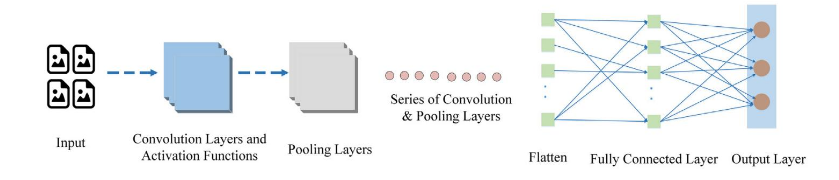
\includegraphics[width=1\linewidth]{lenet5.png}
	\caption{Архитектура LeNet-5}
	\label{templ:image11}
\end{figure}

Существенный прорыв в развитии сверточных сетей произошел, когда была разработана AlexNet в 2012 году. Она выиграла соревнование ImageNet, сократив ошибку классификации почти вдвое по сравнению с предыдущими моделями. AlexNet глубже использовала сверточные архитектуры, функцию активации ReLU, нормализацию по пакету и технику «дропаут» для уменьшения переобучения. Эта модель показала эффективность свёрточных сетей и стала катализатором их развития в целом. На рисунке ~\ref{templ:image12} представлена архитектура AlexNet.
\begin{figure}[h]
	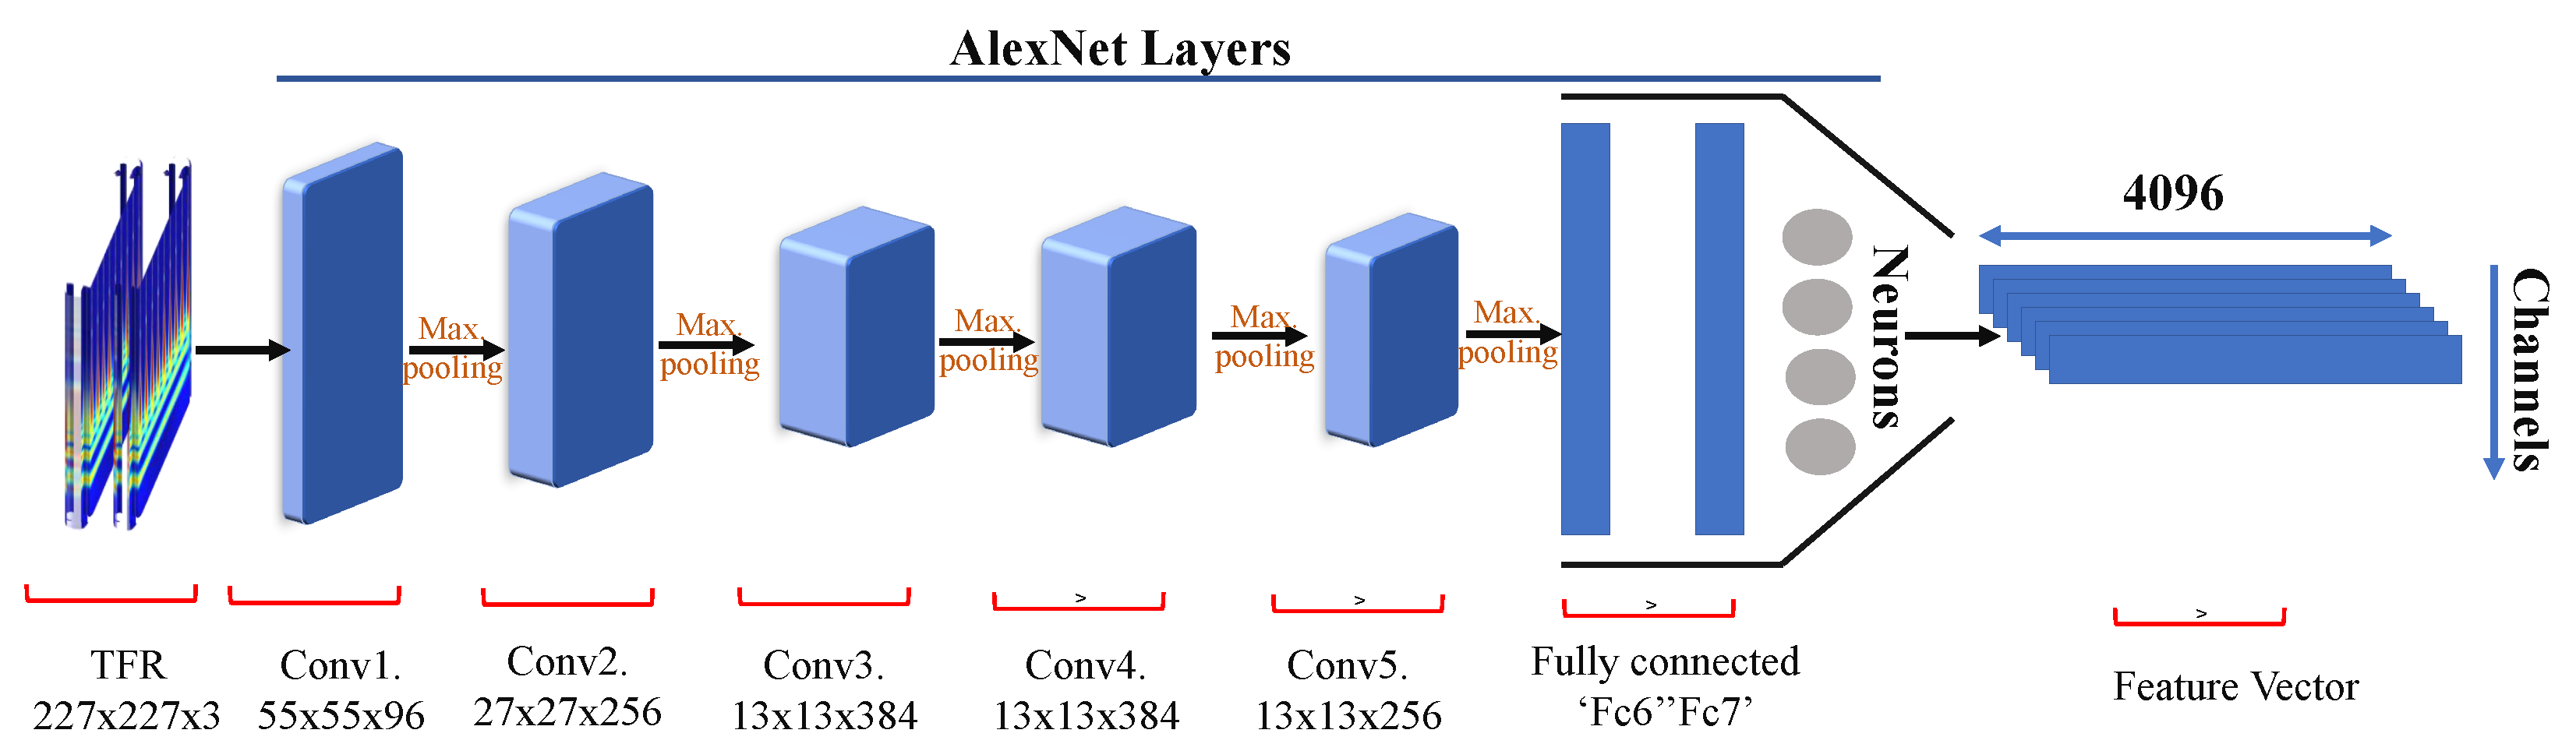
\includegraphics[width=1\linewidth]{alexnet.png}
	\caption{Архитектура AlexNet}
	\label{templ:image12}
\end{figure}

Впоследствии были разработаны более глубокие и эффективные архитектуры, такие как VGG, в которой использовались только 3×3 свёрток и 2×2 пуллинга, ResNet, в которой введены остаточные связи для облегчения обучения очень глубоких сетей, и GoogLeNet, которая использовала модули Inception. Эти модели стали стандартом в компьютерном зрении. Они применяются в различных отраслях: от медицины и промышленной диагностики до систем анализа спутниковых снимков. 

Развитие CNN позволило перейти от задач классификации к задачам более высокого уровня сложности, в частности к сегментации. Суть этой задачи заключается в построении пиксельных масок, которые соответствуют различным объектам или классам на изображении. Такой подход позволил расширить функциональность моделей по сравнению с обычной классификацией. Примерами соответствующих архитектур являются U-Net, DeepLab и Mask R-CNN, каждая из которых использует комбинацию сверточных и деконволюционных операций, а также механизмы пропуска слоев и многоуровневого объединения признаков \cite{d22}  .

Одним из ключевых направлений в развитии методов компьютерного зрения стало обнаружение объектов. Данная задача предполагает совместное решение задач классификации и локализации. Модель при этом должна не только определить принадлежность объекта к определённому классу, но и задать его пространственные координаты на изображении.

Для её  решения были разработаны архитектуры, сочетающие высокую производительность и точность. Наиболее известными моделями являются YOLO (You Only Look Once), SSD (Single Shot Multibox Detector) и Faster R-CNN. 

Первая из них представляет собой одноэтапную архитектуру. Она осуществляет предсказание координат и классов объектов в рамках единой свёрточной сети. Благодаря своей архитектуре, отличается высокой вычислительной эффективностью и возможностью обработки изображений в режиме, близком к реальному времени. 

Модель SSD тоже основана на одноэтапном подходе. Она использует многомасштабные карты признаков для распознавания объектов различных размеров, что делает её более универсальной при работе с разнородными данными. 

Faster R-CNN имеет двухэтапную архитектуру. Первый модуль генерирует предложений о потенциальной области объектов, а второй выполняет классификацию. Такой подход обеспечивает высокую точность за счёт явного разделения этапов локализации и распознавания.

\subsection{Анализ основных видов заболеваний томатов}

Томаты (Solanum lycopersicum) -- это одна из ключевых овощных культур, которую выращивают во всём мире. Она широко используется при приготовлении пищи и обладает высокой агрономической значимостью. В 2023 году мировое производство томатов составило более 190 млн тонн \cite{plant12}. Это показывает устойчивую тенденцию роста, даже на фоне климатических и биотических стрессов.

Однако томаты подвержены значительным потерям урожая из-за болезней и вредителей. Потери могут достигать 50\% в условиях высокой заболеваемости, особенно при отсутствии своевременного выявления заболеваний \cite{plant14} .

Одной из таких болезней является альтернариоз, или сухая пятнистость листьев. Это грибковое заболевание, вызываемое патогенами рода Alternaria, преимущественно Alternaria solani и Alternaria tomatophila. Заболевание поражает листья, стебли, плоды и приводит к значительным потерям урожая. 

Первые признаки болезни проявляются на нижних листьях в виде небольших тёмно-коричневых пятен с концентрическими кольцами. Со временем пятна увеличиваются, сливаются и охватывают большую часть листовой поверхности, вызывая преждевременное отмирание листьев. На стеблях и черешках появляются продольные тёмные полосы, которые могут приводить к их растрескиванию. На плодах появляются пятна гнили болотного цвета. 

Развитию болезни способствуют: высокая влажность воздуха, температура в диапозоне от +20$^{\circ}$C до +30$^{\circ}$C, густая посадка, мешающая циркуляции воздуха. Споры гриба могут сохраняться в почве и на растительных остатках до 2–3 лет, поэтому необходимо соблюдать севооборот и тщательно убирать поля после сбора урожая \cite{plant2}. На рисунке ~\ref{templ:image1} представлены признаки болезни на листьях.
\begin{figure}[h]
	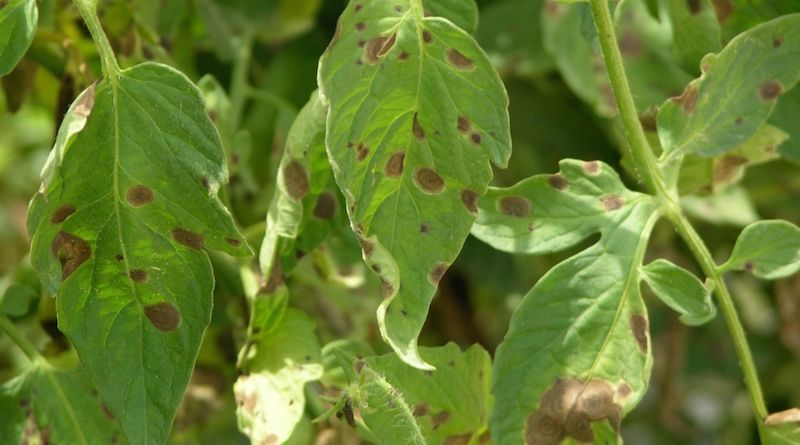
\includegraphics[width=1\linewidth]{альтерниоз tomatov.jpg}
	\caption{Альтернариоз}
	\label{templ:image1}
\end{figure}

Одним из наиболее опасных заболеваний томатов является фитофтороз, вызываемый оомицетом Phytophthora infestans. Эта патогенная микроскопическая структура также поражает картофель и другие растения семейства паслёновых. Фитофтороз способен стремительно распространяться в условиях высокой влажности и умеренных температур, вызывая массовое заражение посадок и значительное снижение урожайности.

Первые признаки заболевания появляются на нижних листьях в виде водянистых пятен бурого или серо-зелёного цвета. По мере развития болезни пятна становятся более выраженными, часть листа вокруг них отмирает, и образуется светлый ободок. С нижней стороны листьев может наблюдаться белый налёт, представляющий собой мицелий патогена. Поражение распространяется вверх по растению. Оно охватывает стебли и плоды. На плодах фитофтороз вызывает бурые, твёрдые пятна, часто с чёрной каймой. Такие плоды быстро загнивают, особенно в условиях хранения \cite{plant3}.
На рисунке ~\ref{templ:image2} представлены признаки болезни на листьях.
\begin{figure}[h]
	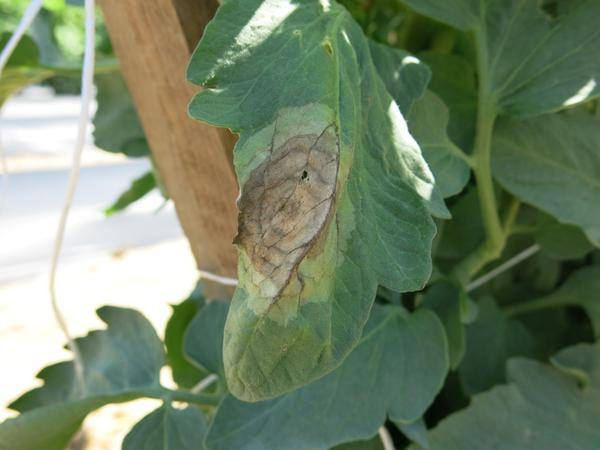
\includegraphics[width=1\linewidth]{late-blight-foliage-tomato.jpg}
	\caption{Фитофтороз}
	\label{templ:image2}
\end{figure}

Кладоспориоз томатов, также известный как бурая пятнистость, — это грибное заболевание. Патоген поражает преимущественно листья томатов, реже -- стебли и плодоножки. У болеющего томата значительно снижается урожайность и качество самих плодов.

Болезнь вызывается грибом Cladosporium fulvum, который развивается на межклеточном уровне и продуцирует токсины, нарушающие физиологические процессы в растении. Грибки распространяется спорами, которые разносятся с потоками воздуха, а также через инструменты, одежду или капли воды. Также источником инфекции могут быть заражённые растительные остатки или семена, не прошедшие предварительную обработку \cite{plant11}.

Наиболее характерные признаки кладоспориоза проявляются на нижней стороне листьев в виде светло-зелёных, жёлтых, а затем бурых пятен округлой или неправильной формы. На рисунке ~\ref{templ:image3} представлено больное растение. Поражённые листья постепенно скручиваются, усыхают и опадают.

\begin{figure}[h]
	
\includegraphics[width=1\linewidth]{кладоспориоз-томата-2-e1598945034942.jpg}
	\caption{Кладоспориоз}
	\label{templ:image3}
\end{figure}

Септориоз томатов, или белая пятнистость, -- это одно из наиболее распространённых грибных заболеваний, вызываемое патогеном Septoria lycopersici Speg. Болезнь поражает преимущественно листву в фазу активного роста растений.

По данным специалистов Россельхозцентра, септориоз регистрируется ежегодно во всех регионах России, но чаще всего в зонах с повышенной влажностью \cite{plant8}.

Первые признаки проявляются на нижних листьях в виде маленьких светло-серых пятен с тёмной каймой. Постепенно пятна увеличиваются до 2–5 мм в диаметре, становятся округлыми, с отчетливо выраженной тёмной границей. В центре пятен можно разглядеть мелкие тёмные точки — пикниды гриба. Изображение больного листа представлено на рисунке ~\ref{templ:image4}.

\begin{figure}[h]
	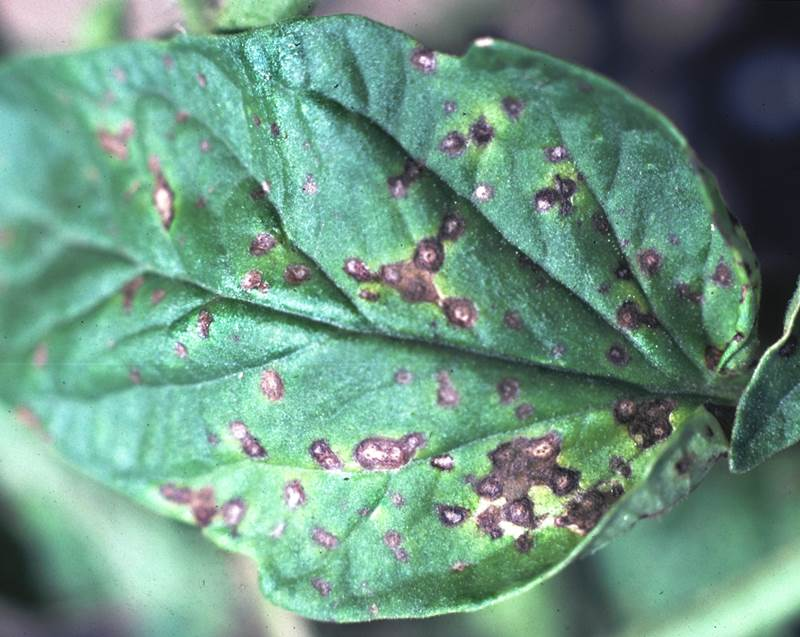
\includegraphics[width=1\linewidth]{4.jpg}
	\caption{Септориоз томата}
	\label{templ:image4}
\end{figure}

При сильном развитии болезни пятна сливаются, листовая пластинка желтеет, высыхает и опадает. Это нарушает фотосинтез и ослабляет растение, особенно в период формирования завязей.

Мозаичный вирус томатов -- одно из наиболее известных и широко распространённых вирусных заболеваний томатов. Болезнь отличается высокой заразностью и может вызвать значительное снижение урожайности и ухудшение качества плодов.

Вирус впервые был описан в начале XX века. Возбудитель относится к роду Tobamovirus и представляет собой устойчивую РНК-вирусную частицу \cite{plant19}.

Первые признаки заражения чаще всего появляются на молодых листьях. Они приобретают характерную мозаичную окраску, при которой чередуются светло-зелёные и тёмно-зелёные участки. На стеблях и черешках появляются бурые полосы, а плоды теряют равномерность окраски и могут быть покрыты кольцевыми пятнами. В условиях высокой температуры и интенсивного солнечного света симптомы становятся более выраженными. Изображение зараженного томата представлено на рисунке ~\ref{templ:image5}.
\begin{figure}[h]
	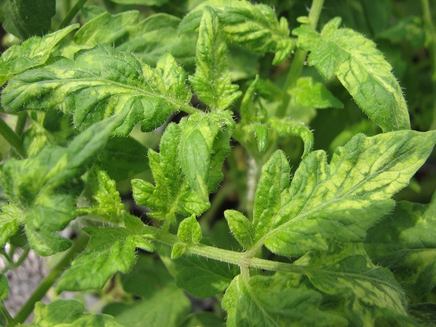
\includegraphics[width=1\linewidth]{pepino-mosaic-virus(4).jpg}
	\caption{Мозаичный вирус}
	\label{templ:image5}
\end{figure}

Передача вируса происходит через контакт с руками, одеждой, садовым инвентарём, на которых есть вирус, или при контакте с насекомыми-переносчиками, такими как тля и табачный трипс \cite{plant5}.

Вирус жёлтой курчавости листьев томата -- ещё одно опасное вирусных заболеваний. Он относится к роду Begomovirus, семейству Geminiviridae, и характеризуется способностью к быстрому распространению, особенно в регионах с тёплым климатом.

На территории России заболевание наиболее часто встречается в южных регионах — Краснодарском крае, Ростовской области, Крыму и Ставрополье, где благоприятные климатические условия способствуют активному размножению основного переносчика -- белокрылки (Bemisia tabaci). Она является единственным распространителем данного вируса \cite{plant13}. Изображение зараженного томата представлено на рисунке ~\ref{templ:image6}.
\begin{figure}[h]
	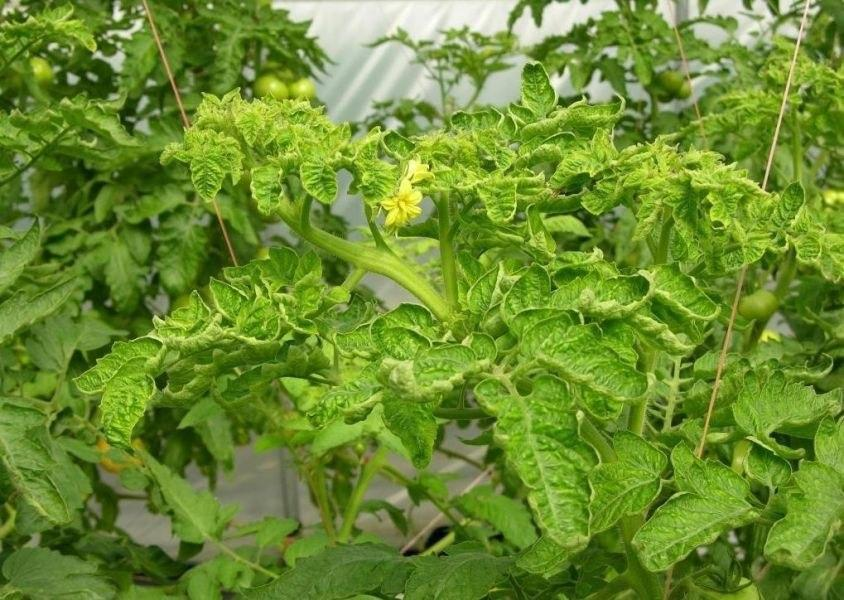
\includegraphics[width=1\linewidth]{Tomato-Yellow-Leaf-4.jpg}
	\caption{Вирус жёлтой курчавости}
	\label{templ:image6}
\end{figure}

У заражённых растений листья уменьшаются в размере, становятся ломкими, закручиваются вверх и приобретают лимонно-жёлтую окраску. Снижается способность к фотосинтезу, и, как следствие, ограничивается формирование цветков и завязей, что приводит к недостаточному развитию плодов или полному отсутствию урожая\cite{plant14}.

Минирующая мушка -- один из опаснейших вредителей овощных культур. Они наносят серьёзный вред растениям, как на стадии рассады, так и в период плодоношения. Эти мелкие двукрылые насекомые относятся к семейству Agromyzidae и отличаются высокой плодовитостью и быстрой адаптацией к инсектицидам. На изображении ~\ref{templ:image7} представлена минирующая мушка \cite{plant15}. 

\begin{figure}[h]
	
\includegraphics[width=1\linewidth]{муха.jpeg}
	\caption{Минирующая мушка}
	\label{templ:image7}
\end{figure}


Самки прокалывают эпидермис листьев для откладки яиц. Вылупившиеся личинки начинают проделывать ходы в мезофилле листа, и, тем самым, разрушают фотосинтетическую ткань. Визуально повреждения проявляются в виде извилистых светлых линий -- мин, которые увеличиваются в размерах по мере роста личинки. Повреждения представлены на изображении ~\ref{templ:image8}. При высокой численности вредителя может быть снижение урожайности до 40\% [ссылка]ФГБУ «Россельхозцентр», 2021).

\begin{figure}[h]
	
\includegraphics[width=1\linewidth]{мин мушка.jpg}
	\caption{"Мины"}
	\label{templ:image8}
\end{figure}

Мушки особенно опасны в теплицах, где температурно-влажностные условия способствуют быстрому размножению. В одном поколении может развиваться до 600–700 яиц, а полный цикл развития при благоприятных условиях занимает 15–20 дней.

Паутинный клещ -- один из наиболее опасных вредителей, поражающих более 200 видов растений, включая томаты. Его биология, малые размеры и высокая устойчивость к пестицидам делают борьбу с ним крайне сложной [ссылка]. Особь клеща представлена на изображении ~\ref{templ:image9}.

Развитие клеща проходит особенно интенсивно при температуре 25–30 $^{\circ}$C и относительной влажности менее 60\%. Полный цикл развития — от яйца до взрослой особи — может занимать всего 7–10 суток, что позволяет вредителю развивать до 20 поколений в год в теплицах. Самки откладывают до 100–150 яиц за жизнь, формируя плотные колонии в межжилковых пространствах листьев \cite{plant18}.

\begin{figure}[h]
	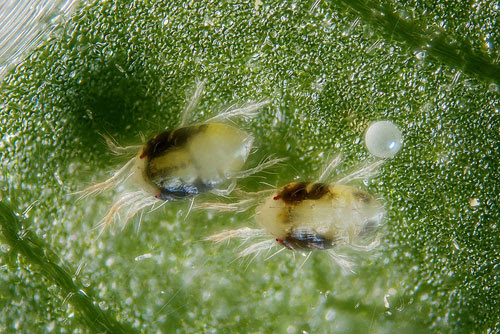
\includegraphics[width=1\linewidth]{клещ.jpg}
	\caption{Паутинный клещ}
	\label{templ:image9}
\end{figure}

На томатах паутинный клещ вредит в основном с нижней стороны листьев, прокалывая эпидермис и высасывая клеточный сок. Первичные симптомы проявляются в виде мелких светлых точек -- хлорозов, которые со временем сливаются и придают листьям мраморный вид. При сильной степени заражения листья буреют, скручиваются, засыхают и опадают. Также можно наблюдать тонкую паутину, покрывающую нижнюю сторону листьев, черешки и даже соцветия. Паутина служит защитой для колоний клещей и яиц от внешних воздействий и инсектицидов [ссылка](Минаев, 2018). На изображении ~\ref{templ:image10} представлен, томатный куст, пострадавший от клещей.

\begin{figure}[H]
	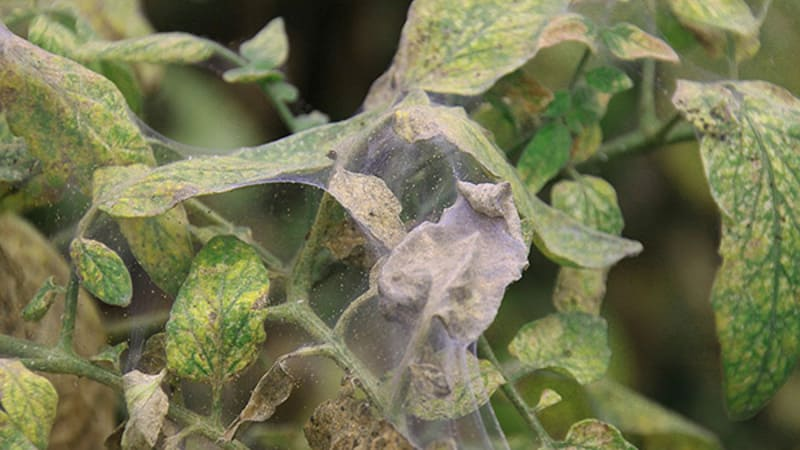
\includegraphics[width=1\linewidth]{паут кл2.jpeg}
	\caption{Колония паутинных клещей на кусте томата}
	\label{templ:image10}
\end{figure}

\subsection{Анализ существующих решений}
С помощью анализу существующих решений с похожей тематикой, можно выделить их достоинства и недостатки, чтобы использовать эту информацию при разработке своего решения. 
Были выбраны три веб-сервиса, в которых используются технологии компьютерного зрения и искусственного интеллекта:
\begin{itemize}
	\item "plantix";
	\item  "cultiKure";
	\item "pdd.jinr".
\end{itemize}
Все указанные платформы решают задачи идентификации болезней растений по загруженным изображениям, однако имеют отличия в интерфейсе, используем технологиях и функционале.

Так Plantix -- это мобильное приложение, ориентированное на фермеров и агрономов. пользователь делает фото растения, а приложение анализирует его и предоставляет подробную информацию о заболевании, методах лечения. Интерфейс рассчитан на массового пользователя и поддерживает множество региональных языков. Однако его минусом является то, что это мобильное приложение, поэтому нет возможности использовать его через браузер. На изображении ~\ref{templ:image13} представлен страница Plantix.

\begin{figure}[ht]
	\centering
	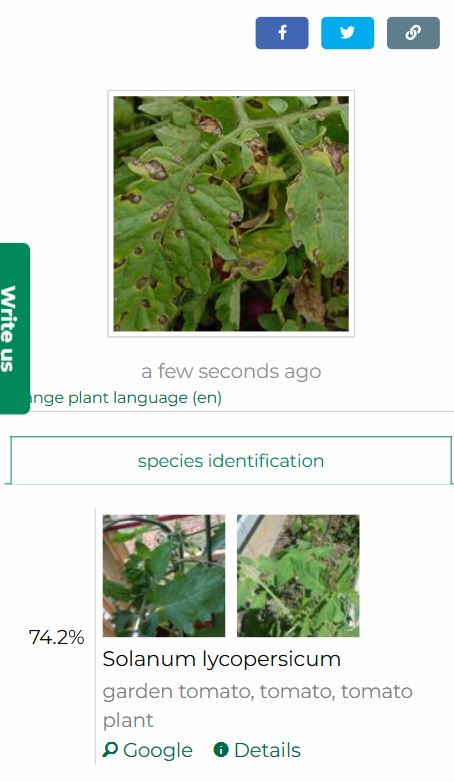
\includegraphics[width=0.5\linewidth]{платекс.png}
	\caption{Интерфейс Plantix}
	\label{templ:image13}
\end{figure}

CultiKure -- это веб-приложение, предназначенное для помощи пользователям в выявлении и устранении заболеваний растений. Оно анализирует изображения листьев с помощью модели VGG16 и выдаёт результаты с информацией по болезням. Само приложение построено на базе фреймворка Flask. Минусом данного решения является то, что оно использует не самую лучшую версию модели, и, как результат, может выдавать не самые точные предсказания \cite{cn1}.
На изображении ~\ref{templ:image14} представлен страница CultiKure.

\begin{figure}[H]
	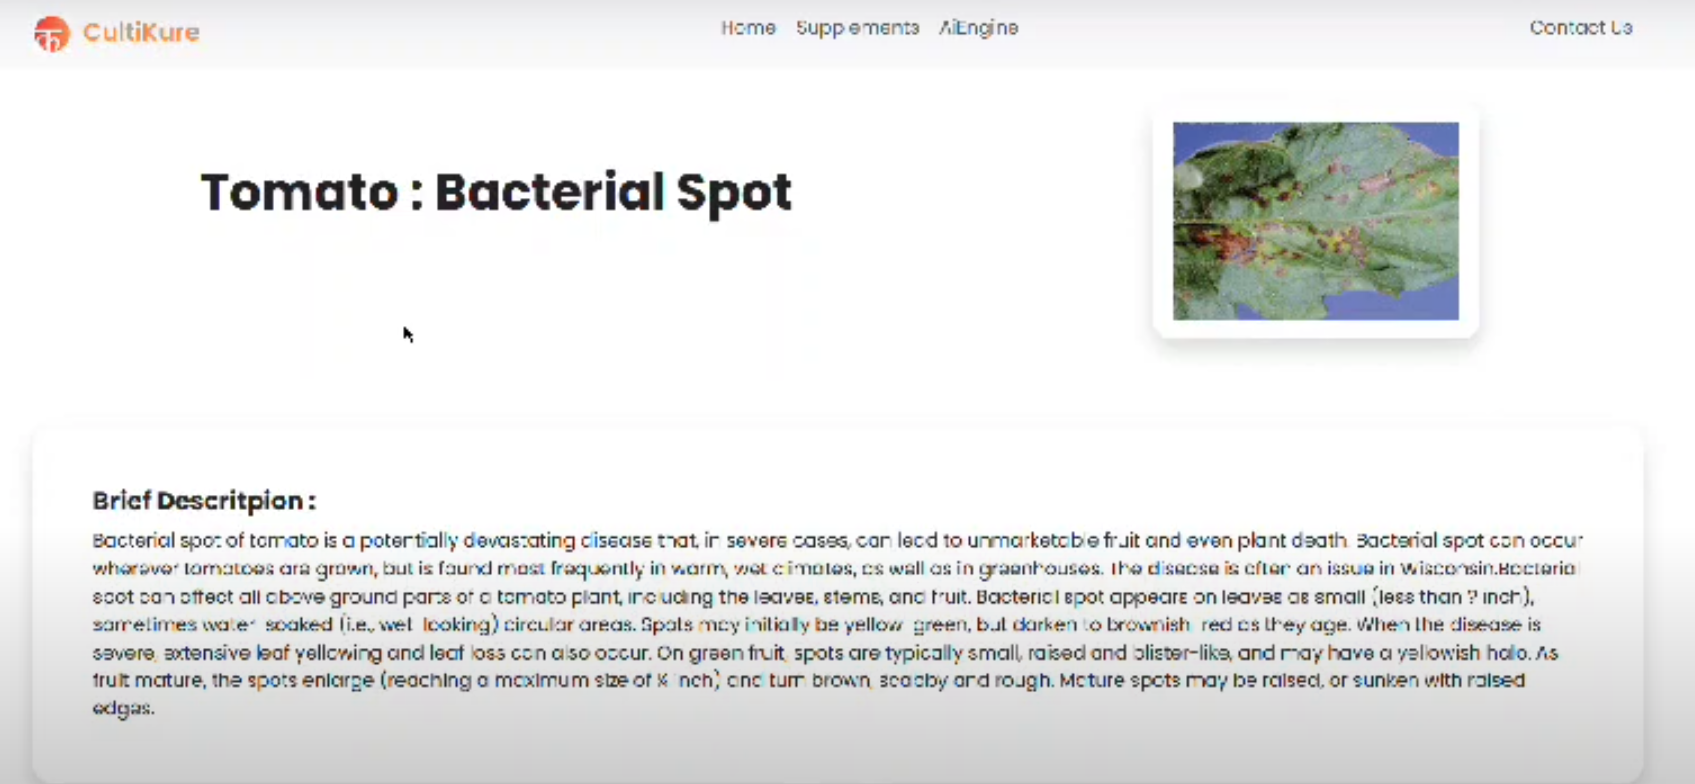
\includegraphics[width=1\linewidth]{култикури.png}
	\caption{Интерфейс CultiKure}
	\label{templ:image14}
\end{figure}

PDD.JINR.RU является исследовательским проектом, созданным в "Объединённом институте ядерных исследований". Веб-интерфейс позволяет загружать изображения листьев и определять заболевание с помощью сверточной нейросети. Акцент данного решения делается на точность и демонстрацию работы алгоритма ИИ. Однако визуальное оформление сайта значительно уступает в удобстве и современности свои конкурентам. На изображении ~\ref{templ:image15} представлен интерфейс, а на ~\ref{templ:image16} - результат предсказания PDD.JINR.RU.

\begin{figure}[H]
	
\includegraphics[width=1\linewidth]{site1.jpg}
	\caption{Интерфейс PDD.JINR.RU}
	\label{templ:image15}
\end{figure}


\begin{figure}[H]
	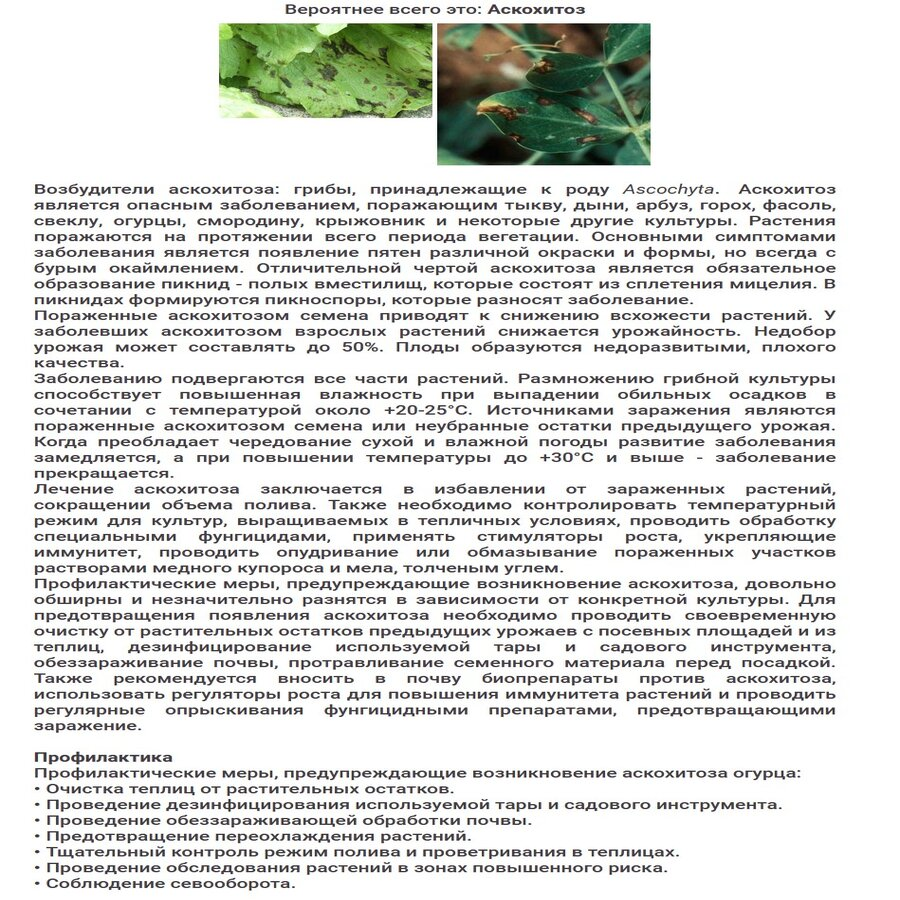
\includegraphics[width=0.9\linewidth]{site2.jpg}
	\caption{Интерфейс PDD.JINR.RU}
	\label{templ:image16}
\end{figure}



\section{Техническое задание}
\subsection{Основание для разработки}

Полное наименование системы: «Разработка интеллектуальной системы для выявления заболеваний сельскохозяйственных растений». Основанием для разработки программы является приказ ректора ЮЗГУ от «17» апреля 2025 г. № 1828-с приказа «О направлении (допуске) на практику». %«Об утверждении тем выпускных квалификационных работ».

\subsection{Цель и назначение разработки}

Программно-информационная система предназначена для диагностики заболеваний томатов по изображениям их листьев. Пользователями системы могут быть как агрономы, так и дачники.

Пользователи должны иметь возможность загружать фотографии поражённой листвы, получать результаты анализа и рекомендации по лечению и профилактике. Кроме того, система должна предоставлять краткое описание выявленного заболевания и возможные причины его возникновения.

Целью разработки является повышение эффективности сельскохозяйственного производства за счёт раннего выявления заболеваний и предоставления точных рекомендаций для их устранения. Это позволит сократить потери урожая, снизить затраты на химическую обработку и улучшить качество плодов.

Задачами данной разработки являются:
\begin{enumerate}
	\item Создание базы данных для хранения информации о заболеваниях, их симптомах, способах лечения и профилактики.
	\item Проектирование пользовательского интерфейса для удобной загрузки изображений и отображения результатов анализа.
	\item Разработка и обучение свёрточной нейросети для точной классификации заболеваний по изображениям.
\end{enumerate}

\subsection{Актуальность темы разработки}

Заболевания растений остаются одной из ключевых проблем в сельском хозяйстве. Они приводят к значительным потерям урожая и снижению его качества, поэтому крайне важной задачей является минимизация потерь за счёт внедрения современных технологий диагностики.

Разработка системы, основанной на использовании свёрточных нейронных сетей для распознавания заболеваний по фотографиям, актуальна по нескольким причинам. Во-первых, она позволяет сократить зависимость от квалификации специалистов, обеспечивая высокую точность диагностики даже для пользователей, которые не разбираются в агрономии. Во-вторых, такая система предоставляет возможность раннего выявления болезней, что существенно увеличивает шансы на успешное лечение. \cite{vkr3}

Кроме того, использование веб-технологий делает решение доступным для пользователей в любых регионах, где есть доступ к сети Интернет. Применение данного подхода может повысить эффективность сельскохозяйственного производства, сократить экономические потери и снизить экологическую нагрузку за счёт оптимизации использования химических средств защиты растений.

В сравнении с традиционными методами диагностики, предложенная система способна в течение нескольких секунд предоставить точный результат анализа, а воспользоваться ею можно везде, где есть Интернет. Эти факторы могут сделать данное решение удобным инструментом для современного сельского хозяйства.

\subsection{Этапы разработки}

Для реализации программной системы предполагается выполнение следующих этапов:
\begin{enumerate}
	\item Изучение существующих решений, определение перечня заболеваний томатов и их визуальных симптомов.
	\item Разработка структуры базы данных для хранения информации о заболеваниях, методах лечения и профилактики.
	\item Сбор и разметка набора данных, обучение модели YOLO 11 и её тестирование.
	\item Создание пользовательского интерфейса, интеграция CNN с веб-приложением.
	\item Проведение функционального тестирования, проверка точности диагностики.
\end{enumerate}

\subsection{Требования к программной системе}

\subsubsection{Требования к данным}
Входными данными для системы являются:
\begin{itemize}
	\item изображения листьев растений, которые пользователь загружает для анализа.
\end{itemize}
Выходными данными для системы являются:
\begin{itemize}
	\item информация о заболевании;
	\item данные об актуальных методах лечения и профилактики;
	\item сообщения об отсутствии информации о заболевании в базе.
\end{itemize}

\subsubsection{Функциональные требования}
Пользователю должны  быть доступны следующие функции:
\begin{itemize}
	\item загрузка фотографии пораженного листа томата для диагностики заболеваний;
	\item просмотр результатов анализа с информацией о выявленном заболевании;
	\item просмотр рекомендаций по лечению;
	\item просмотр информации по профилактике.
\end{itemize}
На рисунке ~\ref{diog1:image} представлена диаграмма прецедентов для пользователя.

\begin{figure}[H]
	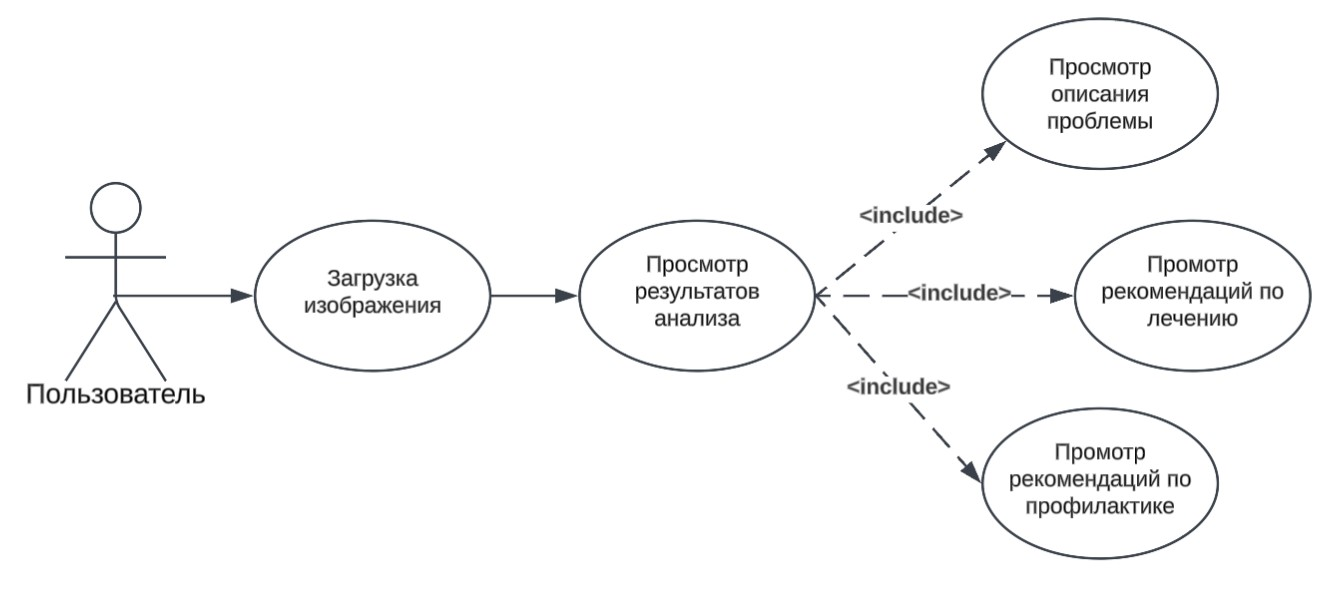
\includegraphics[width=1\linewidth]{diog1}
	\caption{Диаграмма прецедентов для пользователя}
	\label{diog1:image}
\end{figure}

\subsubsection{Сценарий прецедента пользователя «Загрузка изображения»}
Основной успешный сценарий:
\begin{itemize}
	\item пользователь заходит на главную страницу системы;
	\item выбирает опцию "Обзор...";
	\item выбирает изображение на своем устройстве;
	\item подтверждает выбор, нажав кнопку "Анализировать изображение";
	\item дожидается завершения анализа.
\end{itemize}

\subsubsection{Сценарий прецедента пользователя «Просмотр описания проблемы»}
Основной успешный сценарий:
\begin{itemize}
	\item изображение проанализировано;
	\item пользователь переходит к параграфу "Описание";
	\item просматривает информацию о найденной проблеме.
\end{itemize}

\subsubsection{Сценарий прецедента пользователя «Просмотр рекомендаций по лечению и профилактике»}
Основной успешный сценарий:
\begin{itemize}
	\item изображение проанализировано;
	\item пользователь переходит к параграфу "Лечение";
	\item просматривает способы устранить проблемы.
\end{itemize}

\subsubsection{Сценарий прецедента пользователя «Просмотр рекомендаций по профилактике»}
Основной успешный сценарий:
\begin{itemize}
	\item изображение проанализировано;
	\item пользователь переходит к параграфу "Профилактика".
	\item просматривает методы профилактики болезни.
\end{itemize}

\subsection{Требования пользователя к интерфейсу web-интерфейса}
Интерфейс должен быть интуитивно понятным, чтобы агрономы и обычные пользователи могли легко взаимодействовать с системой.
На рисунке ~\ref{maksite1:image} представлен макет страницы.

\begin{figure}[H]
	\centering
	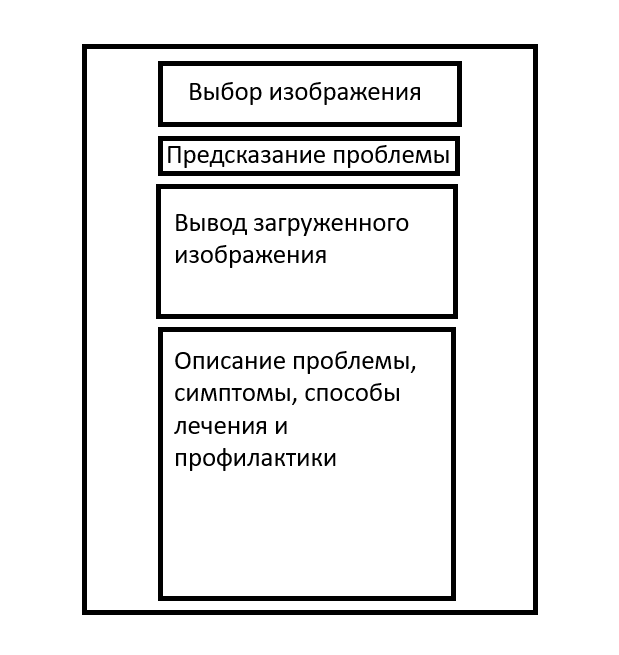
\includegraphics[width=0.9\linewidth]{макет изображения.png}
	\caption{Макет страницы}
	\label{maksite1:image}
\end{figure}

\subsection{Нефункциональные требования}

\subsubsection{Требования к программному обеспечению}

Для разработки и работы программной системы необходимы следующие компоненты:
\begin{itemize}
	\item среда разработки Python для реализации и настройки алгоритмов;
	\item фреймворк Flask для создания веб-приложения;
	\item СУБД PostgreSQL для хранения данных о пользователях, результатах анализа и рекомендациях;
	\item инструменты машинного обучения Ultralytics и Pytorch для работы с CNN;
	\item библиотеки OpenCV, PIL для обработки изображений и Pandas, NumPy для работы с данными.
\end{itemize}

Предлагаемые технологии поддерживаются на всех популярных операционных системах, таких как Windows, macOS и Linux \cite{python1}. Выбор таких инструментов обусловлен их гибкостью, производительностью и большим сообществом разработчиков, что упрощает разработку и последующую поддержку системы.

\subsection{Ограничения}

\begin{enumerate}
	\item Система ориентирована на диагностику заболеваний томатов и не поддерживает другие культуры, поэтому может выдавать ошибочные предположения при загрузке изображений других культур.
	\item Точность диагностики зависит от качества предоставленных входных данных.
	\item Для работы системы требуется стабильное интернет-соединение.
\end{enumerate}

\subsubsection{Требования к аппаратному обеспечению}
Для работы приложения требуется дисковое пространство не менее 2,5 Гб, минимум 2 Гб оперативной памяти и подключение к Интернету. Рекомендуется использовать процессор c 2 или более ядрами и частотой 2 ГГц или выше.

\subsection{Требования к оформлению документации}

Разработка программной документации и программного изделия должна производиться согласно ГОСТ 19.102-77 и ГОСТ 34.601-90. Единая система программной документации.

\section{Технический проект}
\subsection{Общая характеристика организации решения задачи}

Задача заключается в разработке интеллектуальной системы для диагностики заболеваний сельскохозяйственных растений, с фокусом на томатах. Система реализована как веб-приложение, которое анализирует изображения листьев, ищет признаки заболеваний с помощью нейросетевой модели YOLOv11 и предоставляет рекомендации по лечению и профилактике. Приложение поможет агрономам и дачникам быстро выявлять болезни растений и принимать меры для сохранения урожая.

\subsection{Обоснование выбора технологии проектирования}

Для создания приложения выбраны технологии, которые обеспечивают высокую производительность, удобство для пользователей и простоту интеграции с моделью машинного обучения.

\subsubsection{Язык программирования Python}

Python -- высокоуровневый язык программирования с динамической типизацией. Его интерпретатор позволяет запускать код на различных платформах, включая Windows, macOS и Linux, без необходимости компиляции. Официальная документация поддерживает разные подходы к программированию, включая процедурный, объектно-ориентированный и функциональный стили, что даёт разработчикам гибкость\cite{python2} \cite{python3}. 

В 2025 году Python остаётся одним из самых популярных языков благодаря своему простому синтаксису и большому количеству  библиотек, которые и позволяют создавать на нём веб-приложения и модели ИИ \cite{python4}\cite{python1}.

\subsubsection{Google Colab}

Google Colaboratory (или просто Colab) -- это бесплатная облачная среда от компании Google для запуска Python-кода. Она позволяет работать с блокнотами Jupyter прямо в браузере, не требуя установки дополнительных программ на компьютер пользователя \cite{colab1}.

Одним из главных преимуществ Colab является доступ к вычислительным ресурсам GPU и TPU, что делает его особенно полезным для обучения и тестирования моделей машинного обучения и нейросетей.

\subsubsection{Фреймворк PyTorch}

PyTorch -- это инструмент, созданный для работы с нейронными сетями на Python. Он используется разработчиками, когда нужно быстро протестировать идею и собрать прототип, особенно в проектах, связанных с машинным обучением. Его ценят за гибкость, читаемость кода и большое количество готовых решений.

Открытый исходный код PyTorch позволяет любому разработчику внести изменения или адаптировать его под собственные задачи. Благодаря этому вокруг проекта сформировалось большое и активное сообщество. Постоянно появляются новые библиотеки, расширения и обучающие материалы, которые делают работу с фреймворком ещё проще \cite{yolo6}.

Среди особенностей -- поддержка как классических, так и продвинутых архитектур нейросетей. Встроенные модули позволяют обрабатывать данные, визуализировать результаты и отслеживать, как ведёт себя модель во время обучения.

Благодаря всему этому PyTorch активно применяется в разных сферах.

\subsubsection{YOLO 11}

YOLOv11 -- это одна из последних разработок в серии алгоритмов для распознавания объектов на изображениях. Эту версию представила команда Ultralytics. Данная модель стала логичным продолжением предыдущих модификаций YOLO, сохранив при этом основной подход: находить и определять объекты за один проход по изображению \cite{yolo8}.

Главное, за что ценят YOLO -- это скорость и точность. Она справляется с обработкой видео и изображений практически в реальном времени. Такая производительность достигается благодаря улучшенной архитектуре сверточной нейросети и доработанному механизму обучения. Разработчики также внедрили более точные методы предобработки данных, что заметно повысило стабильность работы модели \cite{yolo2}. 

На изображении ~\ref{graf:image} представлены результаты сравнения 11-ой версии с предшествующими ей. 

\begin{figure}[H]
	\centering
	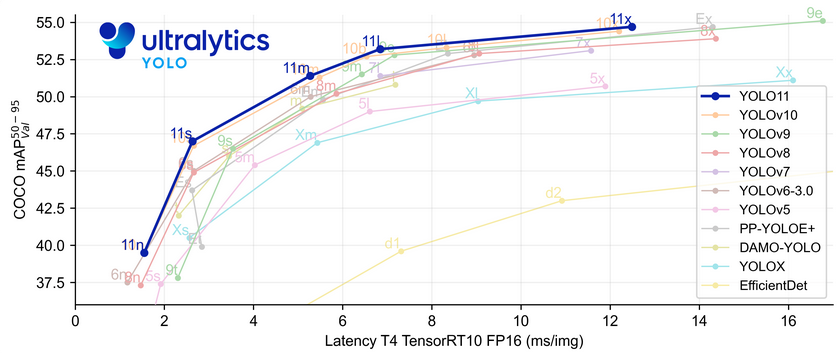
\includegraphics[width=1\linewidth]{garfYolo.png}
	\caption{График сравнения версий YOLO}
	\label{graf:image}
\end{figure}

\subsubsection{Фреймворк Flask}

Flask -- это легковесный веб-фреймворк на языке Python, который часто используют для разработки простых и понятных веб-приложений. Он не навязывает структуру проекта, поэтому подойдёт как новичкам, так и разработчикам, которым нужен контроль над архитектурой \cite{flask1}.

В отличие от более тяжёлых решений, Flask не включает в себя избыточных модулей. Вместо этого он предлагает только базовые инструменты -- маршрутизацию, работу с запросами и шаблонизатор \cite{flask2}.

Для разработки веб-интерфейса системы распознавания заболеваний растений Flask подойдёт особенно хорошо. Он позволяет быстро реализовать обработку изображений, вывод результатов и взаимодействие с нейросетью. Благодаря простому синтаксису и большому количеству обучающей информации, с реализацией приложений не возникает серьёзных трудностей, даже при ограниченном опыте в веб-программировании \cite{flask4}.

Фреймворк хорошо работает на любых операционных системах и легко разворачивается как на локальной машине, так и на сервере. Это делает Flask удобным выбором для небольших и средних проектов.

\subsubsection{PostgreSQL}

PostgreSQL -- это СУБД с открытым исходным кодом. Она известна своей стабильностью, надёжностью и соответствием стандартам SQL \cite{postgres1}.

PostgreSQL активно используется как в небольших проектах, так и в крупных корпоративных системах. Среди её ключевых особенностей -- поддержка сложных запросов, транзакций, расширяемость и работа с JSON-данными. Это делает её удобной для современных веб-приложений \cite{postgres2}.

В этой работе PostgreSQL используется для хранения данных о болезнях растений, их признаках и рекомендациях по лечению.

\subsection{Архитектура программной системы}

На рисунке \ref{comp:image} показана архитектура программной системы.
 
 \begin{figure}[ht]
 	\center{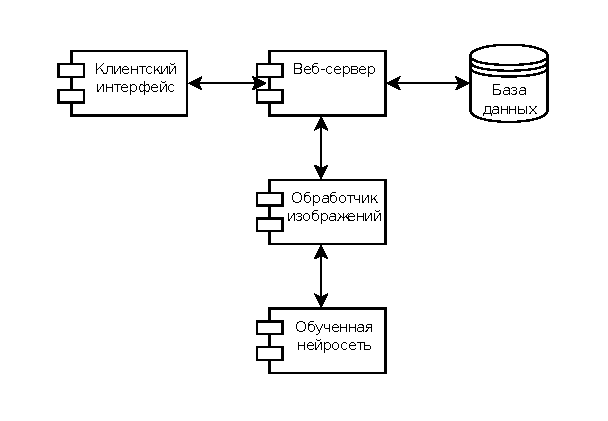
\includegraphics[width=1\linewidth]{Компоненты.eps}}
 	\caption{Диаграмма компонентов}
 	\label{comp:image}
 \end{figure}
 
 Диаграмма показывает, как устроено веб-приложение для диагностики заболеваний томатов. Она представлена в виде схемы с пятью основными блоками, соединёнными стрелками. Они указывают, как данные передаются между частями приложения. Каждая часть выполняет свою задачу, чтобы обеспечить работу системы.
 
 Клиентский интерфейс -- это веб-страница, через которую пользователь загружает изображение листьев. На этой же странице он видит результат анализа.%: найденный недуг, советы по его устранению и методы для профилактики.
 
 Веб-сервер стоит в центре схемы и управляет всем процессом. Он принимает запросы от интерфейса, направляет данные в нужные модули и возвращает результат пользователю. 
 
 База данных хранит описание болезней томатов, методы лечения, способы профилактики. Сервер обращается к ней, если модель нашла недуг.
 
 Модуль обработки изображений подготавливает загруженное фото для анализа. Он изменяет размер изображения, повышает резкость и контраст, а затем передаёт его в модель. 
 
 Нейронная сеть анализирует изображение и определяет, есть ли на фото болезнь и возвращает на сервер результат.

\subsubsection{Архитектура нейронной сети}
Основным параметром сети является nc, который указывает, сколько классов модель может распознавать. Для решаемой задачи устанавливаем nc равное 9. 

Далее задаём варианты масштабирования, которые регулируют глубину, ширину сети и максимальное число каналов. Будем использовать глубину 0.50, ширину 0.25 и максимум 1024 канала. Данная модель состоит из 181 слоя и 2,624,080 параметров.

Архитектура YOLOv11 делится на три основные части: Backbone, Neck и Head. Они представлена на схеме ~\ref{йоло:image}.
\begin{landscape}
	\begin{figure}[p]
		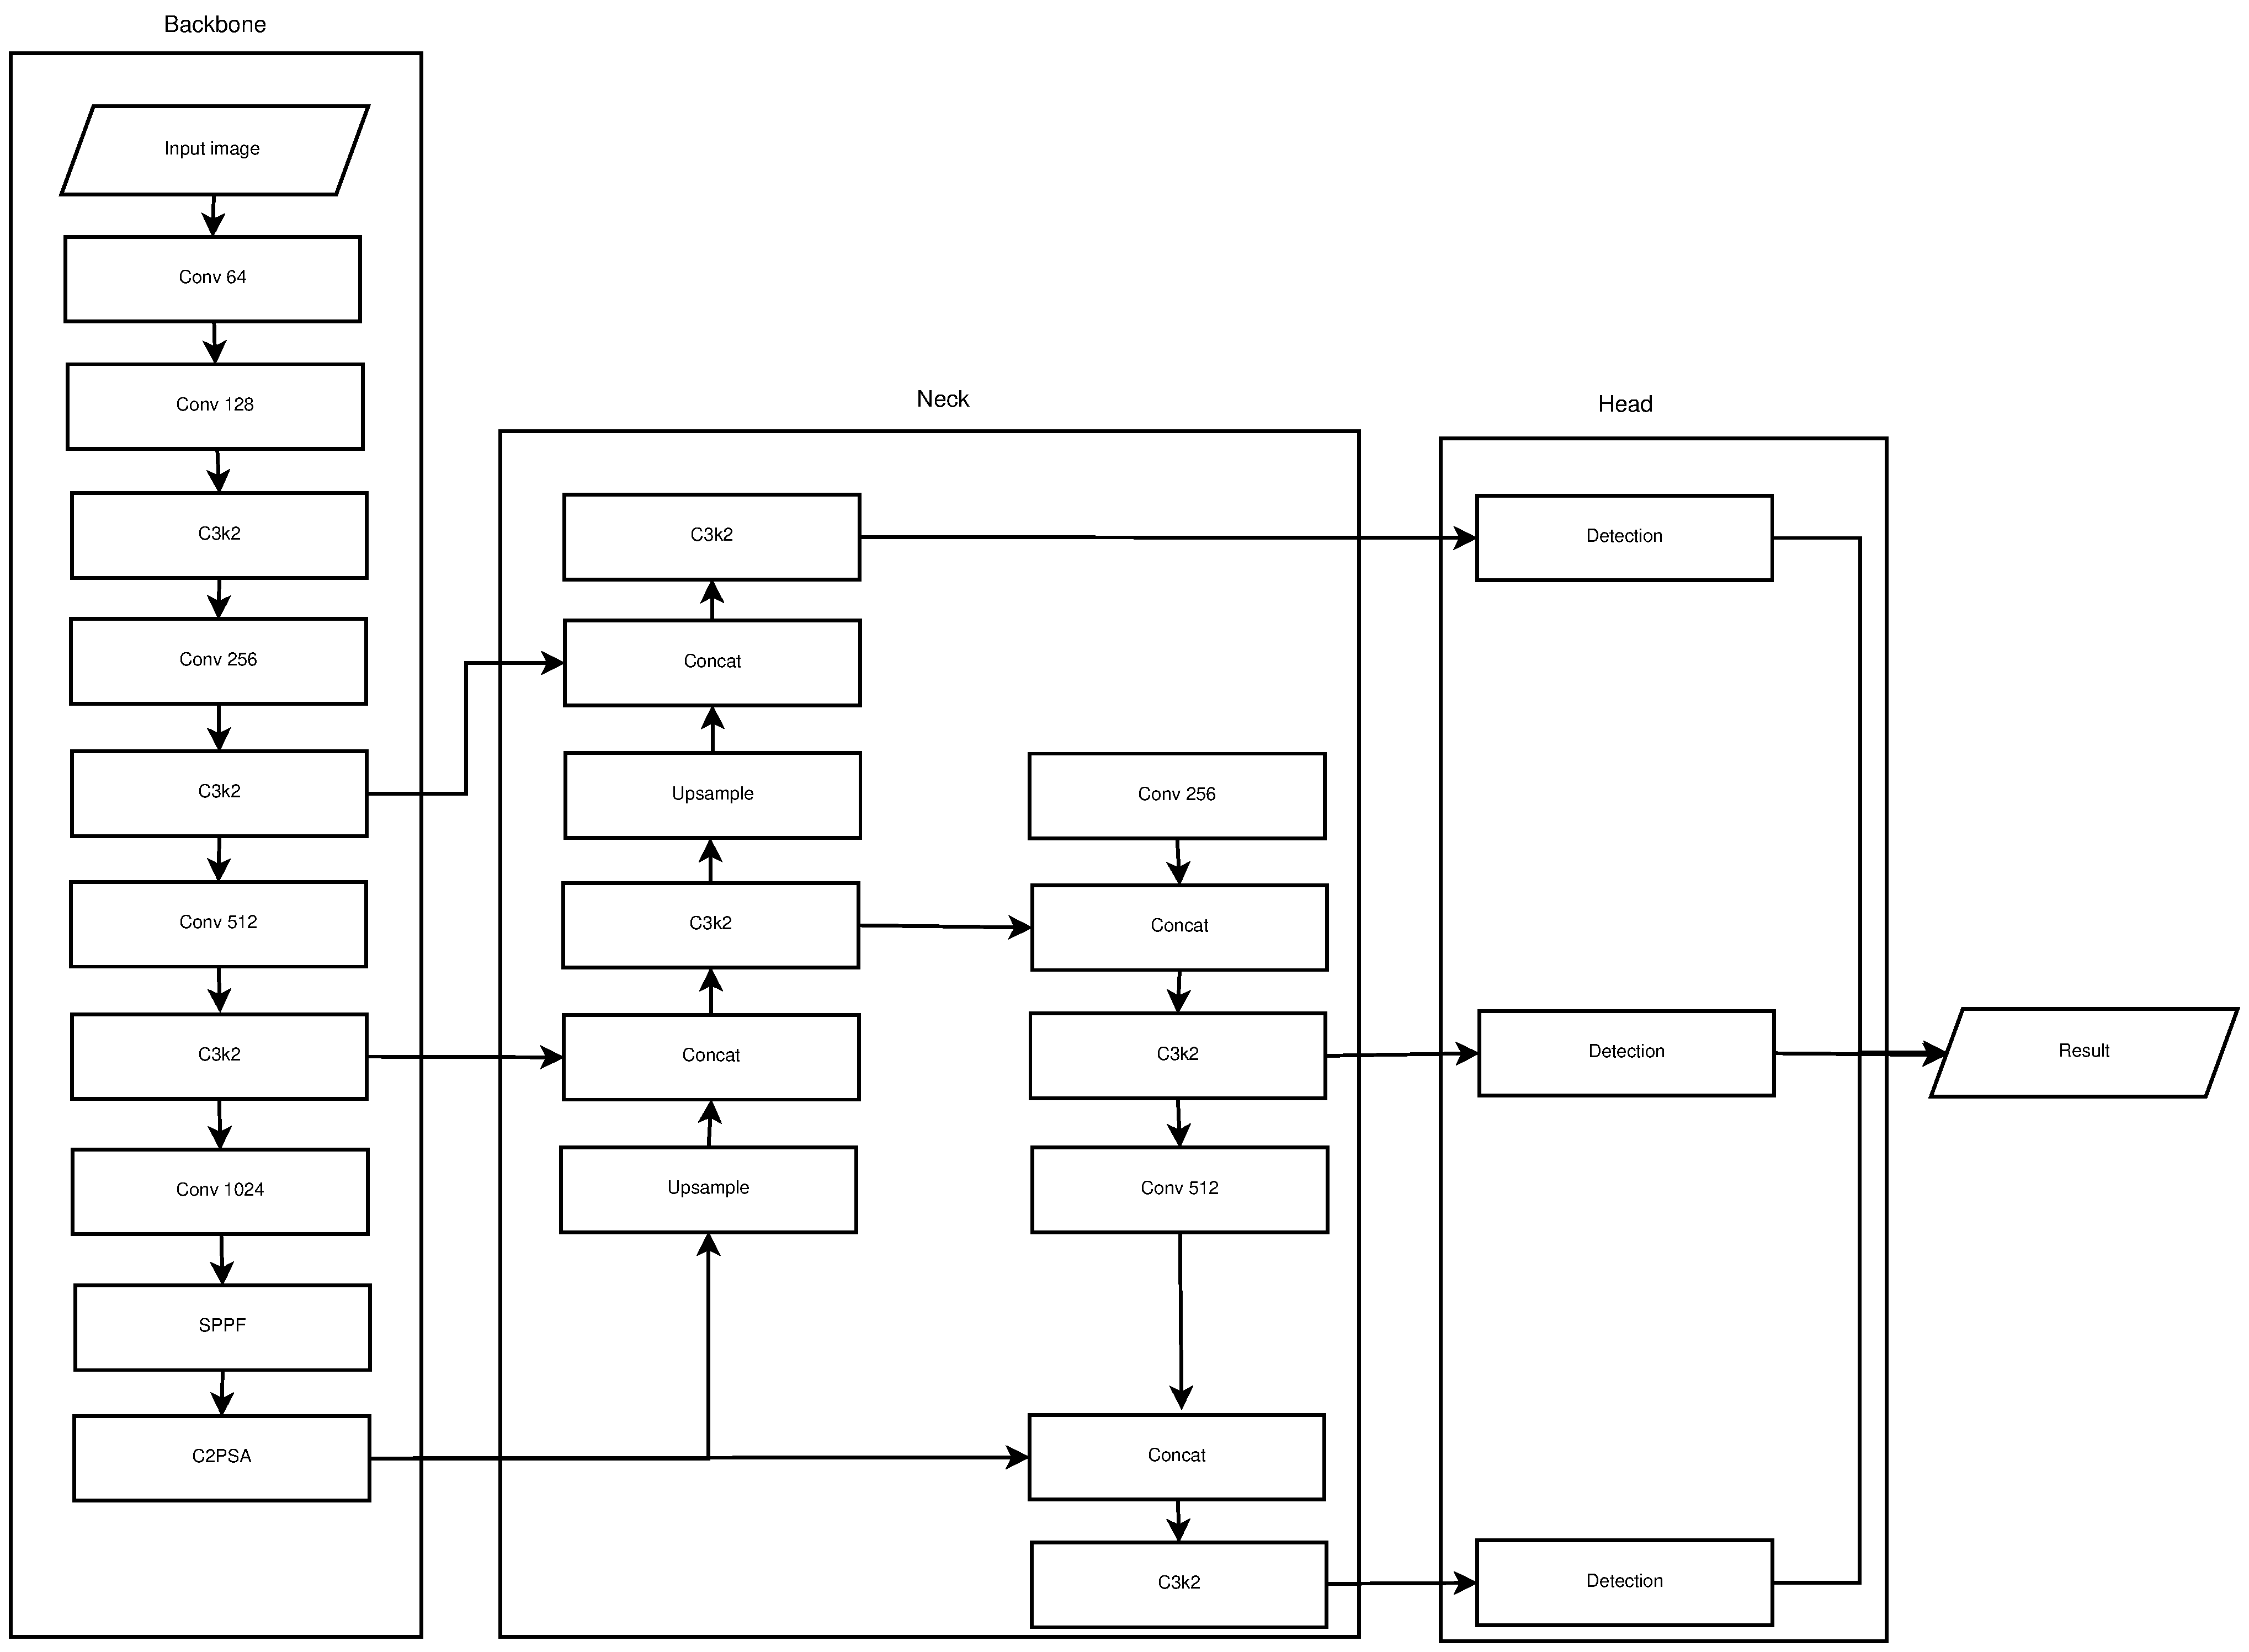
\includegraphics[width=1.05\linewidth, height=0.65\linewidth]{Yolo.eps}
		\caption{Архитектура YOLO 11}
		\label{йоло:image}
	\end{figure}
\end{landscape}
\paragraph{Backbone}

Backbone анализирует входное изображение размером 640x640 пикселей. Основной его задачей является выделение важных деталей, таких как края, текстуры или пятна на листе, которые характерны для заболеваний. Архитектура Backbone постепенно уменьшает размер изображения и увеличивает глубину признаков через следующие слои \cite{yolo8}:

\begin{enumerate}
	\item Conv 64 -- свёрточный слой с 64 фильтрами размером 3x3 и шагом 2, он уменьшает изображение с 640x640x3 до 320x320x64. При свёртке идёт обобщение крупных структур, таких как контуры листьев.
	
	\item Conv 128 -- свёрточный слой с 128 фильтрами размером 3x3 и шагом 2 уменьшает размер до 160x160x128, усиливая выделение текстурных особенностей.
	
	\item C3k2 -- улучшенный блок C3 с двумя свёрточными слоями и остаточными связями, которые пропускают часть входных данных через блок без изменений и добавляют их к выходу. Это предотвращает проблему затухающего градиента во время обратного распространения. На выходе имеем изображение 160x160x256.
	
	\item Conv 256 уменьшает размер до 80x80x256, фокусируясь на признаках средней детализации, таких как пятна 10–20 пикселей.
	
	\item Блок C3k2 с двумя свёрточными слоями преобразует данные до 80x80x512, выделяя более сложные текстуры, такие как пятна или повреждения листьев.
	
	\item Слой conv 512 формирует карту размером 40x40x512, фокусируется на объектах среднего размера.
	
	\item Блок C3k2 сохраняет размер 40x40x512, углубляет признаки.
	
	\item Conv 1024 формирует карту размером 20x20x1024, выделяет крупные области поражения.
	
	\item Блок C3k2 сохраняет размер 20x20x1024, углубляет признаки.
	
	\item SPPF применяет пулинг с разными масштабами ядер (5x5, 9x9, 13x13), чтобы захватить признаки разной детализации. В отличие от других методов пулинга, SPPF ускоряет этот процесс за счёт оптимизированных свёрток.
	 
	\item C2PSA основан на механизме само-внимания, который оценивает взаимосвязи между разными частями изображения. Это помогает модели сосредотачиваться на важных областях, таких как мелкие пятна или изменения цвета, игнорируя фоновые элементы.
	
\end{enumerate}

Backbone формирует карты признаков 80x80x256, 40x40x512, 20x20x1024 и передаёт  в neck.

\paragraph{Neck}

Neck собирает данные из backbone и готовит их к финальному этапу детекции. Эта часть объединяет информацию с разными масштабами, чтобы модель могла лучше находить мелкие объекты. Neck состоит из следующих модулей \cite{yolo3}:

\begin{enumerate}
	\item Слой Upsample преобразует 20x20x1024 в 40x40x1024, используя интерполяцию, что улучшает анализ мелких деталей.
	
	\item Слой Concat соединяет 40x40x1024 с 40x40x512, формируя 40x40x1536. Это помогает сделать карту признаков полнее.  

	\item Блок C3k2 преобразует 40x40x1536 в 40x40x512, углубляет признаки.
	
	\item Upsample преобразует 40x40x512 в 80x80x512, что улучшает анализ мелких объектов.
	
	\item Слой Concat формирует 80x80x768, соединяя 80x80x512 с 80x80x256.
	
	\item C3k2 выдаёт 80x80x256, углубляет признаки.
	
	\item Слой Conv 256 преобразует 80x80x256 в 40x40x256 и подготавливает данные для следующего масштаба.
	
	\item Concat соединяет 40x40x256 с 40x40x512 и формирует 40x40x768.
	
	\item Блок C3k2 выдаёт 40x40x512, углубляет признаки.
	
	\item Conv 512 преобразует 40x40x512 в 20x20x512.
	
	\item Concat формирует 20x20x1536, соединяя 20x20x512 с 20x20x1024. 
	
	\item C3k2 выдаёт 20x20x1024, углубляет признаки.

\end{enumerate}

Neck готовит три карты признаков размерностями 80x80x256, 40x40x512 и 20x20x1024 и отправляет их в head для диагностики.

\paragraph{Head}

Head -- это последняя часть модели, которая выдаёт результаты на основе данных из neck. Блок Detect обрабатывает каждый масштаб и делает предсказания координат рамок, вероятностей классов и уверенности. Он использует свёртки, чтобы получить эти данные.

\subsection{Структура модулей программы}

Программа для диагностики заболеваний томатов представляет собой веб-приложение, реализованное с использованием Python, модели YOLO11 для обнаружения болезней, PostgreSQL для хранения данных и HTML/CSS для клиентского интерфейса. Структура программы организована в виде набора модулей, каждый из которых выполняет определённые функции. На схеме ~\ref{модули:image} представлена структура разрабатываемого решения.
	\begin{figure}[H]
		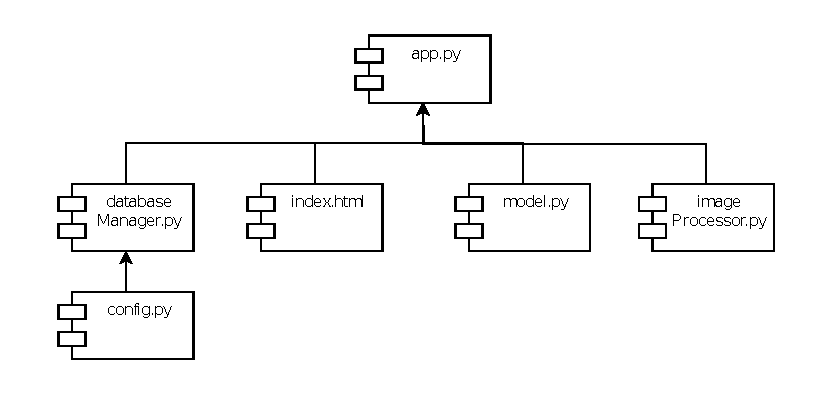
\includegraphics[width=1\linewidth]{Modules.eps}
		\caption{Структура модулей программы}
		\label{модули:image}
	\end{figure}

\begin{enumerate}
	\item Модуль app.py 
	Основной файл серверной части, реализованный на фреймворке Flask. Обрабатывает GET и POST запросы для загрузки изображений, кодирует изображения в base64 для отображения и запрашивает данные о болезни из базы данных.
	
	\item Модуль databaseManager.py
	Модуль для взаимодействия с базой данных PostgreSQL. Содержит класс Database для настройки соединения с базой, выполняет SQL-запросы для получения данных о болезни, включая методы лечения и профилактики.
	
	\item Модуль config.py
	Файл конфигурации, содержащий параметры подключения к базе данных.
	
	\item index.html
	HTML-шаблон клиентского интерфейса. Содержит форму для загрузки изображений, блок для отображения данных о болезни. Использует CSS-стили из файла styles.css.
	
	\item Модуль model.py. Загружает и настраивает обученную модель для анализ изображений и выявление заболеваний.
	
	\item Модуль imageProcessor.py. выполняет предварительную обработку изображений для анализа моделью и их преобразование для отображения в интерфейсе.
	
\end{enumerate}

\subsection{Структура базы данных}

Сущности и отношения между ними отображены на ER-диаграмме.

 \begin{figure}[ht]
	\center{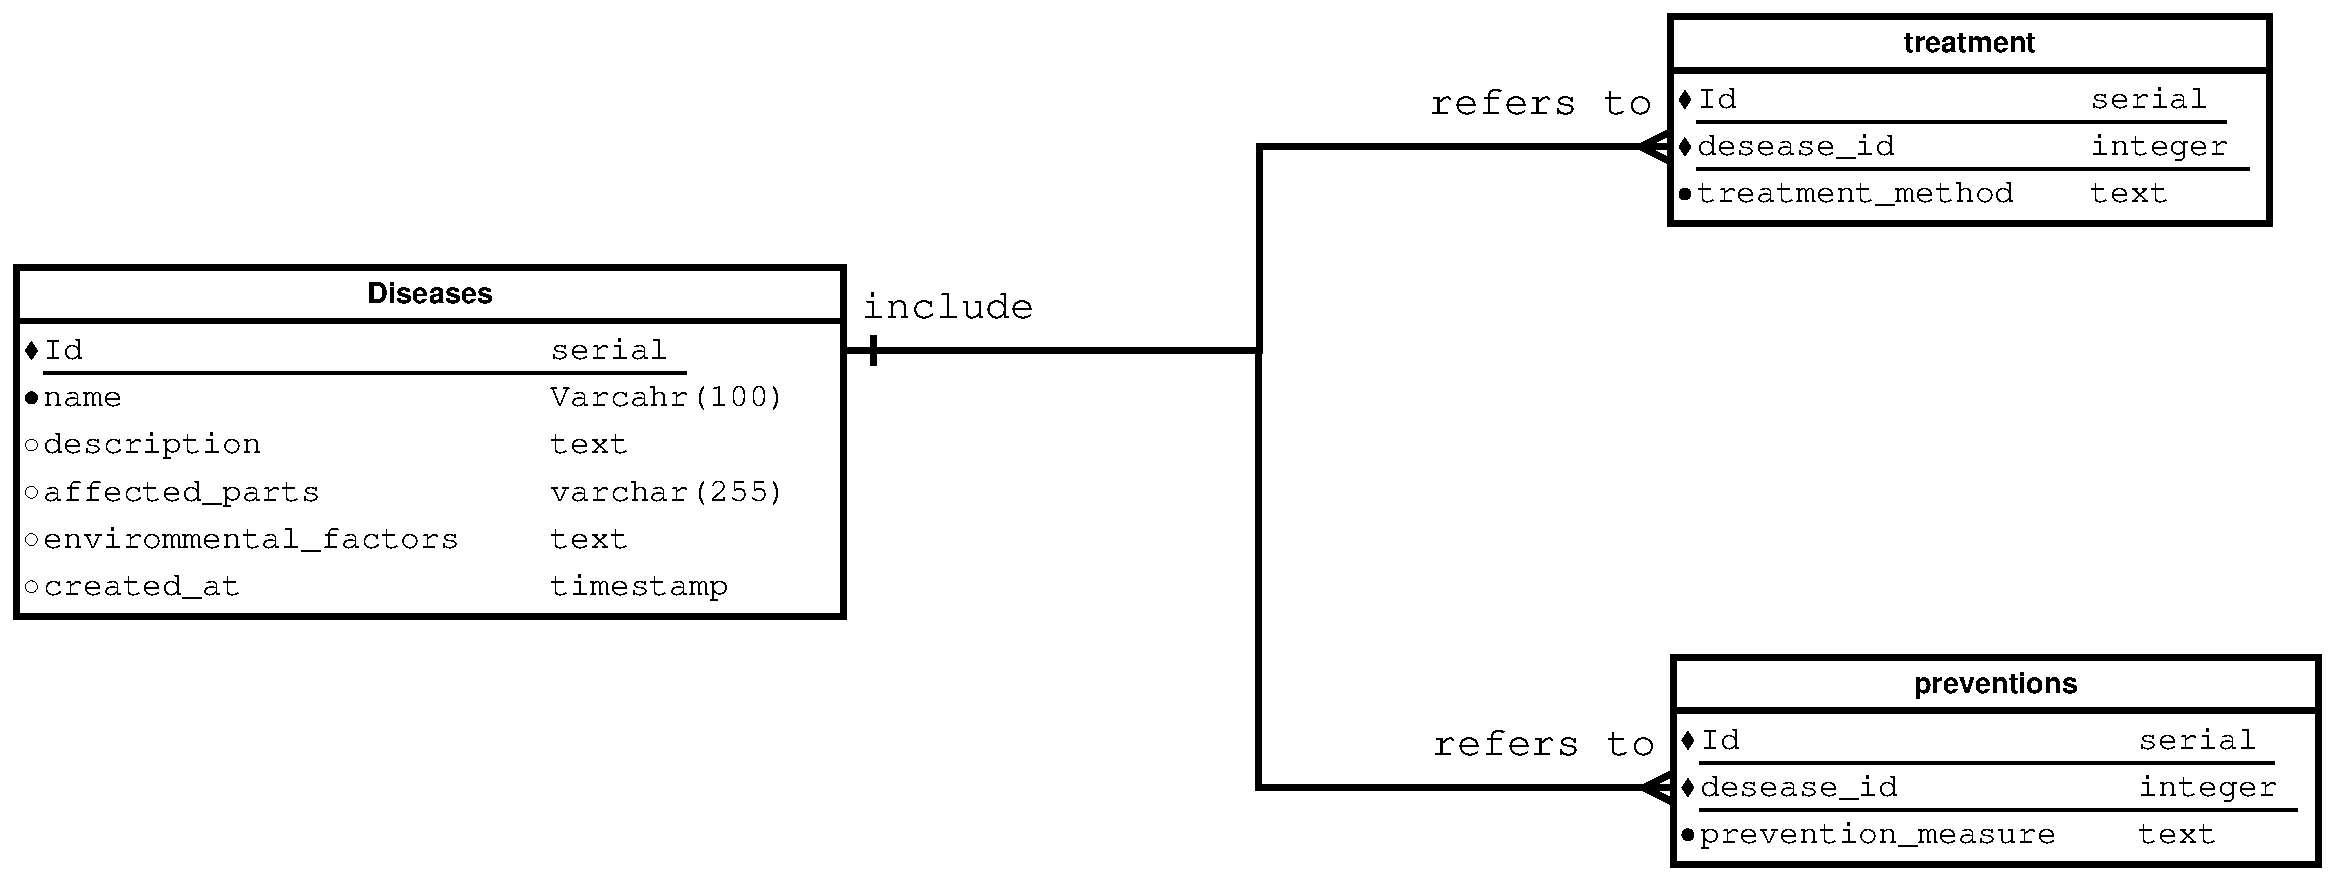
\includegraphics[width=1\linewidth, height=0.5\linewidth]{ДиаграммаБд}}
	\caption{ER-диаграмма}
	\label{er:image}
\end{figure}


\begin{xltabular}{\textwidth}{|l|l|p{1.7cm}|X|}
	\caption{Атрибуты сущности diseases\label{diseases:table}}\\ \hline
	\centrow Поле & \centrow Тип & \centrow Обяза\-тельное & \centrow Описание \\ \hline
	\thead{1} & \thead{2} & \centrow 3 & \centrow 4 \\ \hline
	\endfirsthead
	\caption*{Продолжение таблицы \ref{diseases:table}} \\ \hline
	\thead{1} & \thead{2} & \centrow 3 & \centrow 4 \\ \hline
	\finishhead
	id & serial & true & Первичный ключт \\ \hline
	name & varchar(100) & true & Название болезни \\ \hline
	description & text & false & Подробное описание болезни \\ \hline
	affected\_parts & varchar(255) & false & Части растения, поражаемые болезнью \\ \hline
	environmental\_factors & text & false & Экологические факторы, способствующие болезни \\ \hline
	created\_at & timestamp & false & Дата и время создания записи \\ \hline
\end{xltabular}

\begin{xltabular}{\textwidth}{|l|l|p{1.7cm}|X|}
	\caption{Атрибуты сущности treatments\label{treatments:table}}\\ \hline
	\centrow Поле & \centrow Тип & \centrow Обяза\-тельное & \centrow Описание \\ \hline
	\thead{1} & \thead{2} & \centrow 3 & \centrow 4 \\ \hline
	\endfirsthead
	\caption*{Продолжение таблицы \ref{treatments:table}} \\ \hline
	\thead{1} & \thead{2} & \centrow 3 & \centrow 4 \\ \hline
	\finishhead
	id & serial & true & Первичный ключ \\ \hline
	disease\_id & integer & true & Внешний ключ, ссылка на таблицу diseases \\ \hline
	treatment\_method & text & true & Описание методов лечения \\ \hline
\end{xltabular}

\begin{xltabular}{\textwidth}{|l|l|p{1.7cm}|X|}
	\caption{Атрибуты сущности preventions\label{preventions:table}}\\ \hline
	\centrow Поле & \centrow Тип & \centrow Обяза\-тельное & \centrow Описание \\ \hline
	\thead{1} & \thead{2} & \centrow 3 & \centrow 4 \\ \hline
	\endfirsthead
	\caption*{Продолжение таблицы \ref{preventions:table}} \\ \hline
	\thead{1} & \thead{2} & \centrow 3 & \centrow 4 \\ \hline
	\finishhead
	id & serial & true & Первичный ключ \\ \hline
	disease\_id & integer & true & Внешний ключ, ссылка на таблицу diseases \\ \hline
	prevention\_measure & text & true & Описание мер профилактики \\ \hline
\end{xltabular}


\ifПрактика{}\else{
   \section{Рабочий проект}
\subsection{Классы, используемые при разработке сайта}

Можно выделить следующий список классов и их методов, использованных при разработке web-приложения (таблица \ref{class:table}). Пример таблицы с уменьшенным межстрочным интервалом.

\renewcommand{\arraystretch}{0.8} % уменьшение расстояний до сетки таблицы
\begin{xltabular}{\textwidth}{|X|p{2.5cm}|>{\setlength{\baselineskip}{0.7\baselineskip}}p{4.85cm}|>{\setlength{\baselineskip}{0.7\baselineskip}}p{4.85cm}|}
\caption{Описание классов Bitrix, используемых в приложении\label{class:table}}\\
\hline \centrow \setlength{\baselineskip}{0.7\baselineskip} Название класса & \centrow \setlength{\baselineskip}{0.7\baselineskip} Модуль, к которому относится класс & \centrow Описание класса & \centrow Методы \\
\hline \centrow 1 & \centrow 2 & \centrow 3 & \centrow 4\\ \hline
\endfirsthead
\caption*{Продолжение таблицы \ref{class:table}}\\
\hline \centrow 1 & \centrow 2 & \centrow 3 & \centrow 4\\ \hline
\finishhead
CMain & Главный модуль & CMain – главный класс страницы web-приложения. После одного из этапов по загрузке страницы в сценарии становится доступным инициализированный системой объект данного класса с именем \$APPLICATION & void ShowTitle(string property\_code = «title», bool strip\_tags = true)
Выводит заголовок страницы
void SetTitle(string title)
Устанавливает заголовок страницы

void ShowCSS(bool external = true, bool XhtmlStyle = true)
Выводит таблицу стилей CSS страницы\\
\hline CFile & Главный модуль & CFile – Класс для работы с файлами и изображениями & array GetFileArray (int file\_id)
Метод возвращает массив, содержащий описание файла (путь к файлу, имя файла, размер) с идентификатором file\_id
\end{xltabular}
\renewcommand{\arraystretch}{1.0} % восстановление сетки

\subsection{Модульное тестирование разработанного web-сайта}

Модульный тест для класса User из модели данных представлен на рисунке \ref{unitUser:image}.

\begin{figure}[ht]
\begin{lstlisting}[language=Python]
from django.test import TestCase
from .models import *
User = get_user_model()


class ShpoTestCases(TestCase):

    def setUp(self) -> None:
        self.user = User.objects.create(username='testtestovich', password='testtestovich', first_name='Sad', last_name='')

    def test_2(self):

        self.assertEqual(self.user.first_name, 'Sad')
        self.assertEqual(self.user.last_name, 'Cat')
        print((self.user))
        print((self.user.first_name))
        print((self.user.last_name))
\end{lstlisting}  
\caption{Модульный тест класса User}
\label{unitUser:image}
\end{figure}

\subsection{Системное тестирование разработанного web-сайта}

На рисунке \ref{main:image} представлена главная страница сайта «Русатом – Аддитивные технологии».
\newpage % при необходимости можно переносить рисунок на новую страницу


На рисунке \ref{menu:image} представлен динамический вывод заголовков, включающий в себя искомые фразы при поиске фраз.



На рисунке \ref{enter:image} представлен ввод данных для публикации новости.


   \section*{ЗАКЛЮЧЕНИЕ}
\addcontentsline{toc}{section}{ЗАКЛЮЧЕНИЕ}

Преимущества аддитивных технологий заключается в разнообразии процессов, позволяющих применять их в различных областях производства. Существенным ограничением же является и экономическая составляющая, которая не позволит внедрить аддитивное производство повсеместно.
  
Компании, видя, как развиваются информационные технологии, пытаются использовать их выгодно для своего бизнеса, запуская свой сайт для того, чтобы заявить о своем существовании, проинформировать потенциального клиента об услугах или продуктах, которые предоставляет. 
Для продвижения компании «Русатом – Аддитивные технологии» был разработан веб-сайт на основе системы «1С-Битрикс: Управление сайтом».

Основные результаты работы:

\begin{enumerate}
\item Проведен анализ предметной области. Выявлена необходимость использовать 1С-Битрикс.
\item Разработана концептуальная модель web-сайта. Разработана модель данных системы. Определены требования к системе.
\item Осуществлено проектирование web-сайта. Разработана архитектура серверной части. Разработан пользовательский интерфейс web-сайта.
\item Реализован и протестирован web-сайт. Проведено модульное и системное тестирование.
\end{enumerate}

Все требования, объявленные в техническом задании, были полностью реализованы, все задачи, поставленные в начале разработки проекта, были также решены.

Готовый рабочий проект представлен адаптивной версткой сайта. Сайт находится в публичном доступе, поскольку опубликован в сети Интернет.  

}\fi
\addcontentsline{toc}{section}{СПИСОК ИСПОЛЬЗОВАННЫХ ИСТОЧНИКОВ}

\begin{thebibliography}{9}
	\bibitem{plant1} Ходж, Д. Ботаника для садоводов / Д. Ходж – Москва~: Азбука-Бизнес, 2024. - 224 с. – ISBN 978-5-389-13415-7. – Текст~: непосредственный.
	
	\bibitem{plant2} Кошкин, Е. И. Патофизиология сельскохозяйственных культур / Е. И. Кошкин – Москва~: РГ-Пресс, 2024. - 304 с. – ISBN 978-5-9988-1405-1. – Текст~: непосредственный.	
	
	\bibitem{plant3} Сергеева, М. Н. Культурные растения / М. Н. Сергеева – Москва~: Проспект, 2023. - 120 с. – ISBN 978-5-392-37362-8. – Текст~: непосредственный.	
	
	\bibitem{plant4} Абросимов, В.К. Интеллектуальные сельскохозяйственные роботы/В.К. Абросимов, А.Н. Райков – Москва~: Карьера Пресс, 2022. - 512 с. – ISBN 978-5-00074-318-8. – Текст~: непосредственный.	

	\bibitem{plant5}  Гриценко, В. В. Меры борьбы с болезнями и вредителями растений в сооружениях защищенного грунта /В. В. Гриценко, И. М. Митюшев, Ю. М. Стройков  – Москва~: Академия, 2020. - 160 с. – ISBN 978-5-44-689434-5. – Текст~: непосредственный.	
	
	\bibitem{plant6} Ерофеева, Т. В. Сельскохозяйственная экология /Ерофеева Т. В., Фадькин Г. Н., Чурилова В. В.  Санкт-Петербург~: Лань, 2025. - 100 с. – ISBN 978-5-507-52249-1. – Текст~: непосредственный.	
	
	\bibitem{plant7} Курбанов, С. А. Сельскохозяйственная мелиорация /С. А. Курбанов  – Санкт-Петербург~: Лань, 2021. - 208 с. – ISBN 978-5-8114-6623-8. – Текст~: непосредственный.	
	
	\bibitem{plant8} Овсинский, И. Е. Новая система земледелия /И. Е. Овсинский  – Москва~: Концептуал, 2023. - 240 с. – ISBN 978-5-907624-99-3. – Текст~: непосредственный.	
	
	\bibitem{sh1} Современное сельское хозяйство : сайт / fnb TECH. – Москва : fnb TECH, 2025 – . – URL: \url{https://fnb.tech/ru/modern-agriculture/} (дата обращения: 23.05.2025). – Текст: электронный.
		
	\bibitem{plant9} Монторо, Ж. Семена и зерна / Ж. Монторо  – Москва~: Эксмо, 2024. - 256 с. – ISBN 978-5-04-196329-3. – Текст~: непосредственный.
	
	\bibitem{plant10}Копытин, И. П. Ведение сельского хозяйства в Центрально-Нечерноземном округе России / И. П. Копытин  – Санкт-Петербург~: Лань, 2022. - 336 с. – ISBN 978-5-8114-9863-5. – Текст~: непосредственный.	
	
	\bibitem{plant11}Савельев, В. А. Растениеводство / В. А. Савельев  – Санкт-Петербург~: Лань, 2021. - 316 с. – ISBN 978-5-8114-8194-1. – Текст~: непосредственный.	
	
	\bibitem{plant12} Ториков, В. Е. Агрономический контроль в растениеводстве / В. Е. Ториков, О. В. Мельникова/ Санкт-Петербург~:Лань, 2024. - 132 с. - ISBN 978-5-507-49427-9. - Текст: непосредственный.
	
	\bibitem{plant13} Ганичкина, О. А. Секреты огородника. Как получить богатый урожай овощей и зелени на вашем участке / О. А. Ганичкина, А. В. Ганичкин  / Москва~:Эксмо, 2024. - 224 с. - ISBN 978-5-04-211846-3. - Текст: непосредственный.
	
	\bibitem{plant14} Кочелаева, Л. Н. Сеньор Помидор. Выращиваем, ухаживаем и едим / Л. Н. Кочелаева  – Москва~: АСТ, 2024. - 160 с. – ISBN 978-5-17-161963-3. – Текст~: непосредственный.	
	
	\bibitem{plant15} Кузнецова, Е. А. Рассадоводство. Первые шаги к здоровому урожаю / Е. А. Кузнецова – Москва: Издательство АСТ, 2023. - 160 с. – ISBN 978-5-17-157334-8. – Текст: непосредственный.
	
	\bibitem{plant16} Ожехелева, З. Е. Биологические препараты для эффективного садоводства / З. Е. Ожехелева – Москва: ФГБНУ ВНИИСПК, 2022. - 166 с. – ISBN 978-5-6049204-3-5. – Текст: непосредственный.
	
	\bibitem{plant17} Кизима, Г. А. Огород и сад для ленивых. Урожаю быть / Г. А. Кизима – Москва: Издательство АСТ, 2020. - 192 с. – ISBN 978-5-17-120651-2. – Текст: непосредственный.
	
	\bibitem{plant18} Волкова, А. П. Энциклопедия пасленовых. Томат. Перец. Баклажан. Физалис / А. П. Волкова – Москва: Издательство АСТ, 2024. - 416 с. – ISBN 978-5-17-164151-1. – Текст: непосредственный.
	
	\bibitem{plant19} Кизима, Г. А. Рассада для начинающих. Первые шаги к богатому урожаю / Г. А. Кизима – Москва: Издательство АСТ, 2025. - 128 с. – ISBN 978-5-17-164591-5. – Текст: непосредственный.
	
	\bibitem{cv20} Демиденко, А. Введение в Computer Vision: как научить компьютер видеть / А. Демиденко – Москва: Литрес, 2025. – 100 с. – ISBN 978-5-04-720541-0. – Текст: непосредственный.
	
	\bibitem{d21} Рутковская, Д. Нейронные сети, генетические алгоритмы и нечеткие системы / Д. Рутковская, М. Пилиньский, Л. Рутковский – Москва: Горячая линия-Телеком, 2023. – 385 с. – ISBN 978-5-9912-0320-3. – Текст: непосредственный.
	
	\bibitem{d22} Лекун, Я. Как учится машина: Революция в области нейронных сетей и глубокого обучения / Я. Лекун – Москва: Альпина PRO, 2021. – 335 с. – ISBN 978-5-907394-92-6. – Текст: непосредственный.
	
    \bibitem{py23} Мэтиз, Э.Изучаем Python: программирование игр, визуализация данных, веб-приложения. 3-е издание / Э. Мэтиз – Санкт-Петербург: БХВ, 2024. – 352 с. – 978-5-9775-1944-1. – Текст: непосредственный.
    
    \bibitem{cv24} Демиденко, А. ИИ и зрение: как машины понимают изображения / А. Демиденко – Москва: Литрес, 2025. – 80 с. – ISBN 978-5-04-727123-1. – Текст: непосредственный.
    
    \bibitem{py25} Любанович, Б. Простой Python / Б. Любанович – Санкт-Петербург: Питер, 2021. – 592 с. – ISBN 978-5-4461-1701-7. – Текст: непосредственный.
    
    \bibitem{cv24} Амундсен, М. RESTful Web API паттерны и практики / А. Демиденко – Москва: Sprint Book, 2025. – 464 с. – ISBN 978-601-08-4867-2. – Текст: непосредственный.
    
	\bibitem{res1} Определитель болезней томатов: фото, описание, меры борьбы и профилактика : сайт / Огород. – Москва : Огород, 2023 – . – URL: \url{https://www.ogorod.ru/ru/ogorod/tomats/14384/Opredelitel-bolezney-tomatov-foto-opisaniye-mery-borby-i-profilaktika.htm} (дата обращения: 13.05.2025). – Текст: электронный.
	
	\bibitem{res2} Болезни рассады томатов: описание с фото, лечение : сайт / КП. – Москва : КП, 2023 – . – URL: \url{https://www.kp.ru/family/sad-i-ogorod/bolezni-rassady-tomatov/} (дата обращения: 13.05.2025). – Текст: электронный.

	\bibitem{yolo1} Распознавание объектов с помощью YOLO v3 на Tensorflow 2.0 : сайт / Proglib. – Москва : Proglib, 2020 – . – URL: \url{https://proglib.io/p/raspoznavanie-obektov-s-pomoshchyu-yolo-v3-na-tensorflow-2-0-2020-11-08} (дата обращения: 13.04.2025). – Текст: электронный.
	
	\bibitem{yolo2} YOLOv11: улучшения в детекции объектов для реального времени : сайт / Ultralytics, 2024 – . – URL: \url{https://docs.ultralytics.com/ru/models/yolo11/} (дата обращения: 13.05.2025). – Текст: электронный.
	
	\bibitem{yolo3} Детекция объектов с помощью YOLOv5 : сайт / Habr. – Москва : Habr, 2021 – . – URL: \url{https://habr.com/ru/articles/576738/} (дата обращения: 11.05.2025). – Текст: электронный.
	
	\bibitem{yolo4} YOLOv7: пользовательское обнаружение объектов : сайт / Habr. – Москва : Habr, 2022 – . – URL: \url{https://habr.com/ru/articles/700794/} (дата обращения: 11.05.2025). – Текст: электронный.
	
	\bibitem{yolo5} Обнаружение объектов с YOLOv3 на Tensorflow 2.0 : сайт / Habr. – Москва : Habr, 2021 – . – URL: \url{https://habr.com/ru/articles/556404/} (дата обращения: 21.04.2025). – Текст: электронный.
	
	\bibitem{yolo6} Как выполнить обнаружение объектов YOLO с помощью OpenCV и PyTorch в Python : сайт / Waksoft. – Челябинск : Waksoft, 2021 – . – URL: \url{https://waksoft.susu.ru/2021/05/19/kak-vypolnit-obnaruzhenie-obektov-yolo-s-pomoshhyu-opencv-i-pytorch-v-python/} (дата обращения: 11.05.2025). – Текст: электронный.
	
	\bibitem{yolo7} Explore Ultralytics YOLOv11 : сайт / Yolov11, 2024 – . – URL: \url{https://yolov11.com/} (дата обращения: 21.04.2025). – Текст: электронный.
	
	\bibitem{yolo8} Как использовать YOLOv11 для обнаружения объектов : сайт / SO Development. – Москва : SO Development, 2024 – . – URL: \url{https://ru.so-development.org/how-to-use-yolov11-for-object-detection/} (дата обращения: 11.05.2025). – Текст: электронный.
	
	\bibitem{yolo9} YOLO11: A New Iteration of “You Only Look Once”: сайт / viso.ai, 2024 – . – URL: \url{https://viso.ai/computer-vision/yolov11/} (дата обращения: 12.05.2025). – Текст: электронный.
	
	\bibitem{yolo10} YOLOv11: настройка и обучение модели для специфичных задач : сайт / Roboflow, 2024 – . – URL: \url{https://roboflow.com/model/yolo11} (дата обращения: 12.05.2025). – Текст: электронный.

	\bibitem{python1} Документация Python: сайт / Habr. – Москва : Habr, 2024 – . – URL: \url{https://www.python.org/doc/} (дата обращения: 02.03.2025). – Текст: электронный.
	
	\bibitem{python2} Язык программирования Python: особенности и перспективы : сайт / GeekBrain. – Москва : GeekBrain, 2024 – . – URL: \url{https://gb.ru/blog/python/} (дата обращения: 14.05.2025). – Текст: электронный.
	
	\bibitem{python3} Обзор языка программирования Python : сайт / Proglib. – Москва : Code Basics, 2023 – . – URL: \url{https://code-basics.com/ru/blog_posts/obzor-yazyka-programmirovaniya-python} (дата обращения: 11.03.2025). – Текст: электронный.
	
	\bibitem{python4} Библиотеки для веб-разработки на Python : сайт / Code Basics. Skypro – Москва : Skypro, 2023 – . – URL: \url{https://sky.pro/wiki/python/biblioteki-dlya-veb-razrabotki-na-python/} (дата обращения: 11.03.2025). – Текст: электронный.
	
	\bibitem{colab1} Google Colaboratory : сайт / Google Colab, 2025 – . – URL: \url{https://colab.google/} (дата обращения: 24.03.2025). – Текст: электронный.

	\bibitem{flask1} Мега-Учебник Flask : сайт / Habr. – Москва : Habr, 2024 – . – URL: \url{https://habr.com/ru/articles/804245/} (дата обращения: 12.03.2025). – Текст: электронный.
	
	\bibitem{flask2} Проектирование RESTful API с помощью Python и Flask : сайт / Skypro. – Москва : Skypro, 20243 – . – URL: \url{https://sky.pro/media/kak-sozdat-rest-api-na-flask/} (дата обращения: 12.03.2025). – Текст: электронный.
	
	\bibitem{flask3} Документация Flask : сайт / Flask, 2020 – . – URL: \url{https://flask.palletsprojects.com/en/stable/} (дата обращения: 14.05.2025). – Текст: электронный.
	
	\bibitem{cn1} Vatathanavaro, S. White Blood Cell Classification: A Comparison between VGG-16 and ResNet-50 Models / V. ЕSupawit, T. Suchat, P. Kitsuchart  – Bangkok~: РГ- King Mongkut’s Institute of Technology Ladkrabang, 2018. - 2 с. – Текст~: электронный – . – URL: \url{https://site.ieee.org/thailand-cis/files/2018/11/JSCI6-Paper-2.pdf} (дата обращения: 11.05.2025).
		
	\bibitem{flask4} Фреймворк Flask: как он работает и зачем нужен : сайт / Skillbox. – Москва : Skillbox, 2023 – . – URL: \url{https://skillbox.ru/media/code/freymvork-flask-kak-on-rabotaet-i-zachem-nuzhen/} (дата обращения: 14.05.2025). – Текст: электронный.
	
	\bibitem{postgres1} Документация PostgreSQL : сайт / Postgresql, 2025 – . – URL: \url{https://www.postgresql.org/docs/} (дата обращения: 11.05.2025). – Текст: электронный.
	
	\bibitem{postgres2} Обзор баз данных PostgreSQL : сайт / Cnews, 2022 – . – URL: \url{https://market.cnews.ru/news/top/2022-04-25_obzor_baz_dannyh_postgresql} (дата обращения: 11.05.2025). – Текст: электронный.
	
	\bibitem{vkr1} ИИ в сельском хозяйстве : сайт / Sber Developer. – Москва : Sber Developer, 2024 – . – URL: \url{https://developers.sber.ru/help/gigachat-api/ai-agricultural} (дата обращения: 14.05.2025). – Текст: электронный.
	
	\bibitem{vkr2} Цифровые технологии и нейросети в сельском хозяйстве : сайт / It фабрика, 2025 – . – URL: \url{https://it-fabric.ru/catalog/neyroseti/tsifrovye-tekhnologii-i-neyroseti-v-selskom-khozyaystve/} (дата обращения: 12.05.2025). – Текст: электронный.
	
	\bibitem{vkr3} Использование машинного обучения и ИИ в сельском хозяйстве : сайт / БиоТех2030. – Москва : БиоТех2030, 2025 – . – URL: \url{http://biotech2030.ru/kak-ii-i-kompyuternoe-zrenie-mogut-sledit-za-rasteniyami/} (дата обращения: 12.05.2025). – Текст: электронный.
	



\end{thebibliography}

\ifВКР{\appendix{Представление графического материала}

Графический материал, выполненный на отдельных листах,
изображен на рисунках А.1--А.\arabic{числоПлакатов}.
\setcounter{числоПлакатов}{0}

\renewcommand{\thefigure}{А.\arabic{figure}} % шаблон номера для плакатов

\begin{landscape}

\begin{плакат}
    
\includegraphics[width=0.82\linewidth]{плакат1.png}
    \заголовок{Сведения о ВКРБ}
    \label{pl1:image}      
\end{плакат}

\begin{плакат}
    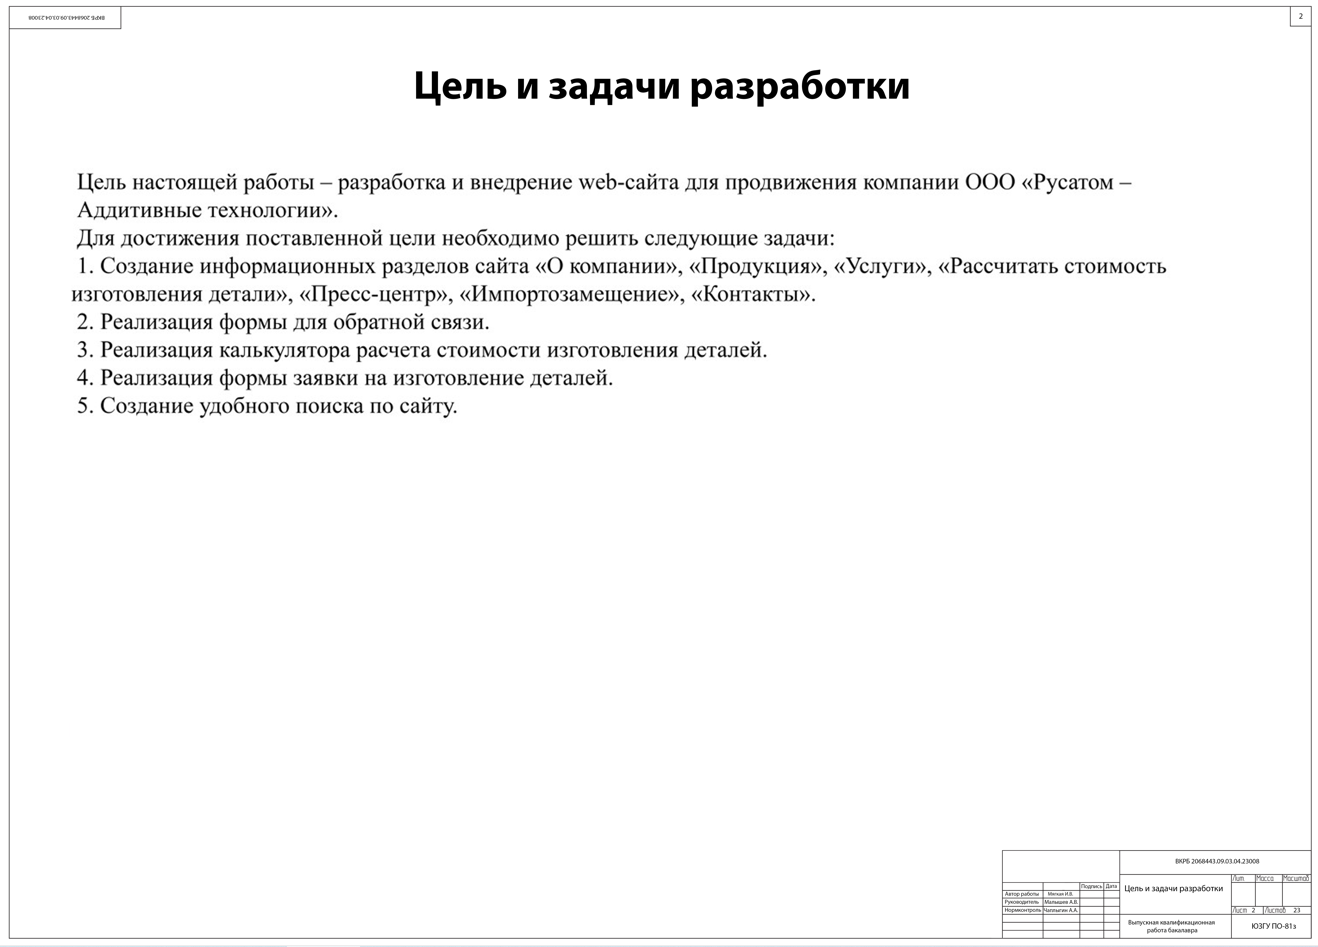
\includegraphics[width=0.82\linewidth]{плакат2.png}
    \заголовок{Цель и задачи разработки}
    \label{pl2:image}      
\end{плакат}

\begin{плакат}
    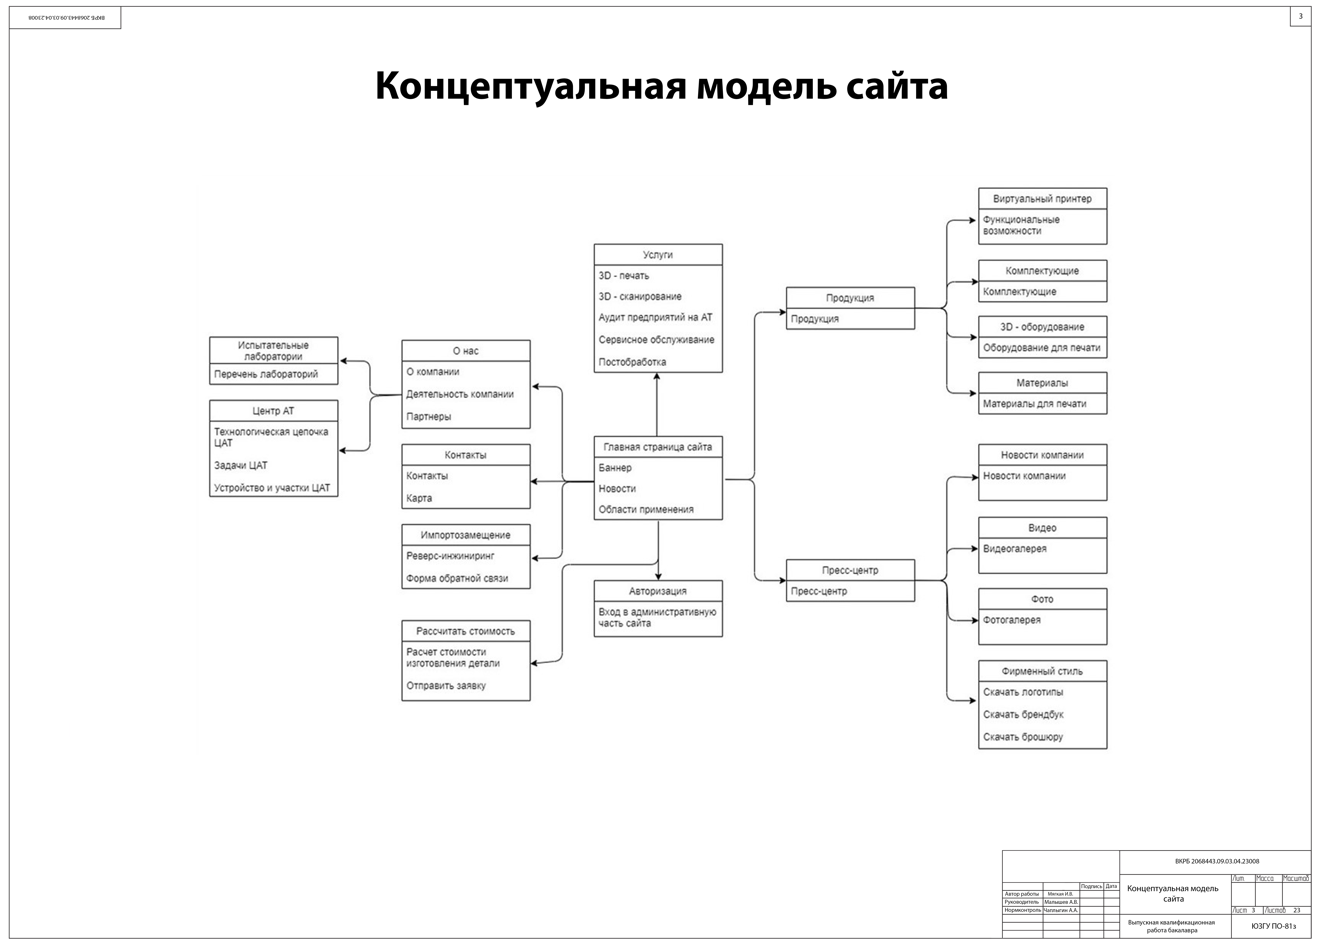
\includegraphics[width=0.82\linewidth]{плакат3.png}
    \заголовок{Концептуальная модель сайта}
    \label{pl3:image}      
\end{плакат}

\begin{плакат}
    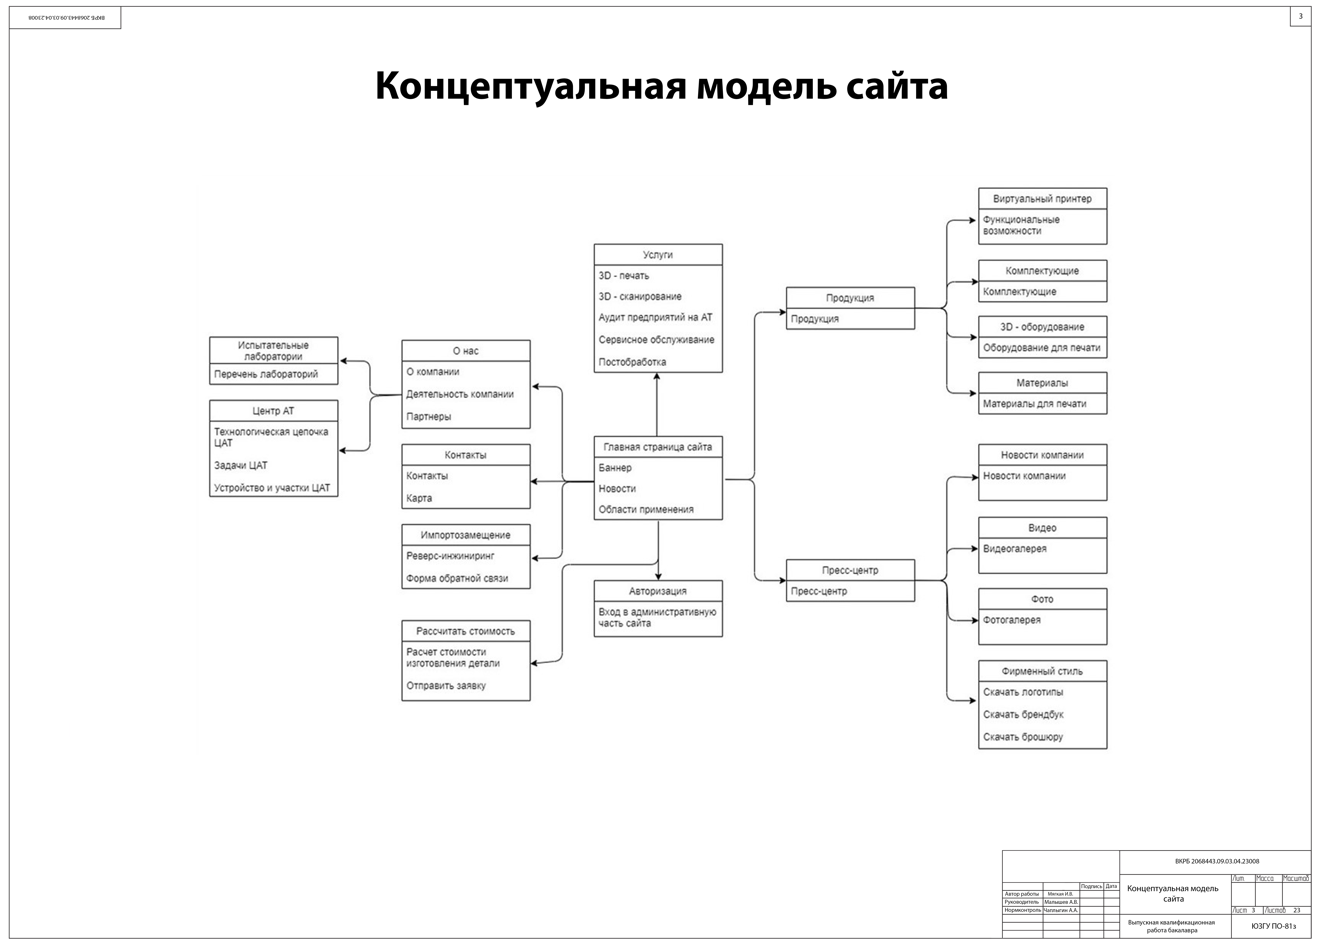
\includegraphics[width=0.82\linewidth]{плакат3.png}
    \заголовок{Еще плакат}
    \label{pl4:image}      
\end{плакат}

\end{landscape}
}\fi
\ifПрактика{}\else{\appendix{Фрагменты исходного кода программы}

main.tex
\lstinputlisting[language=Tex, frame=none]{main.tex}

%ТехПроект.tex
%lstinputlisting[language=Tex, frame=none]{ТехПроект.tex}

\ifВКР{
\newpage
\addcontentsline{toc}{section}{На отдельных листах (CD-RW в прикрепленном конверте)}
\noindent
\begin{tabular}{p{5.8cm}C{4.8cm}C{4.8cm}}
   Автор ВКР & \lhrulefill{\fill} & \fillcenter\Автор \\
            \setarstrut{\footnotesize}
           & \footnotesize{(подпись, дата)} & \\
            \restorearstrut
   Руководитель ВКР & \lhrulefill{\fill} & \fillcenter\Руководитель \\
            \setarstrut{\footnotesize}
           & \footnotesize{(подпись, дата)} & \\
            \restorearstrut
   Нормоконтроль & \lhrulefill{\fill} & \fillcenter\Нормоконтроль \\
            \setarstrut{\footnotesize}
           & \footnotesize{(подпись, дата)} & \\
            \restorearstrut
\end{tabular}
\vskip 2cm
\begin{center}
\textbf{Место для диска}
\end{center}
}\fi
}\fi
\end{document}
